\documentclass[11pt]{iopart}
\usepackage{graphicx}
\usepackage{subfig}
\usepackage{hyperref}
\usepackage{lineno}
\usepackage{booktabs}
% Let us use amsmath.
\expandafter\let\csname equation*\endcsname\relax
\expandafter\let\csname endequation*\endcsname\relax
% Let us use amsmath.
\usepackage{amsmath,isomath,amssymb,bm}
\usepackage[noabbrev]{cleveref}
\usepackage[section]{placeins}
\usepackage{algorithm}
\usepackage{algpseudocode}
\usepackage{comment}
\usepackage[sort&compress,numbers]{natbib}
\usepackage{algorithm}
\usepackage{algpseudocode} % Package for algorithm typesetting (pseudo-code).
\usepackage{lmodern}
\graphicspath{{./images/}}
\renewcommand{\vec}{\vectorsym}
\newcommand{\tns}{\tensorsym}
\newcommand{\mtx}{\mathbf}
\newcommand{\hvar}[1]{\ensuremath{^{\textrm{h}}#1}}
\newcommand{\dvar}[1]{\ensuremath{^{\textrm{d}}#1}}
\newcommand{\tvar}[1]{\ensuremath{^{\textrm{t}}#1}}
\newcommand{\rvar}[1]{\ensuremath{\textrm{#1}}}
\newcommand{\nn}{\nonumber\\}							% No number skip line.
\algblockdefx[gpufunction]{GPUFunction}{EndGPUFunction}%
[2][]{\textbf{GPU function} \textsc{#1}(#2)}%
{\textbf{end GPU function}}

\begin{document}
%% Title, authors and addresses
\title{Accurate evaluation of dislocation tractions}
\author[]{Daniel Celis-Garza, Edmund Tarleton}

\ead{edmund.tarleton@materials.ox.ac.uk}

\address{Department of Materials, University of Oxford, Parks Road, OX1 3PH, UK}

\begin{abstract}
    %% Text of abstract
    Dislocations generate tractions on the surface of a finite volume. Traditionally the dislocation tractions are integrated numerically over a finite element face to obtain the nodal forces; as required when using superposition to couple discrete dislocation plasticity and the finite element method. Here we implement analytic finite element nodal forces obtained using closed form expressions for the traction integrals. We compare the behaviour of the errors which arise when using numerical integration, provide insight into how and why they occur and give recommendations on avoiding numerical issues when implementing the analytic solution. Evaluating the tractions analytically in a large scale discrete dislocation plasticity simulations of a microcantilever showed a clear difference in the simulated load-displacement curve while the dislocation structure was unchanged.
\end{abstract}

%%
%% Start line numbering here if you want
%%
%\linenumbers

%% main text
\section{Introduction}\label{s:intro}

Coupling discrete dislocation dynamics (DDD) to the finite element method (FEM) allows micromechanical tests to be simulated \cite{Groh2009}. Virtual experiments are essential for interpreting experimental data and relating the measured mechanical response to dislocation mechanisms \cite{0965-0393-6-6-007,doi:10.1080/14786430500341250,tarleton2015discrete,YU2018}. One of the most popular methods for coupling DDD and FEM is the superposition method \cite{superposition_scheme0,superposition_scheme1,superposition_scheme2}.
%
\begin{figure}
    \centering
    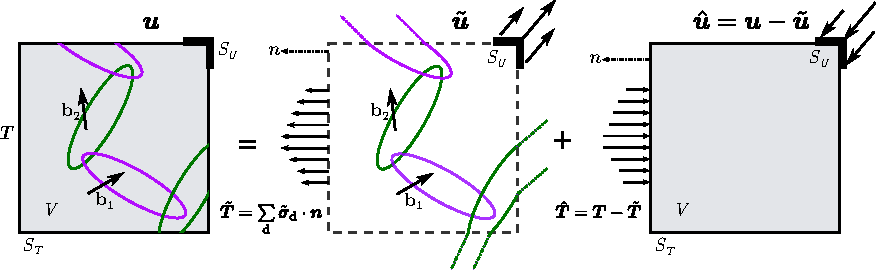
\includegraphics[width=\linewidth]{fem_ddd.pdf}
    \caption[Superposition Model for DDD-FEM coupling.]{The superposition used to couple DDD and FEM. The volume $V$ is bounded by a surface $S = S_{T} \cup S_{U}$ and contains a dislocation ensemble and is subjected to tractions $\vec{T}$ on $S_{T}$ and $\vec{u}$ on $S_{u}$. First, the traction, $\vec{\tilde{T}}$, and displacement, $\vec{\tilde{U}}$, fields due to the dislocations in the infinite domain (DDD) are evaluated on the boundaries $S_{T}$ and $S_{U}$ respectively. Then an elastic boundary value problem can be solved with FEM to calculate the corrective elastic fields required to satisfy the boundary conditions $\vec{\hat{T}} = \vec{T} - \vec{\tilde{T}}$ and $\vec{\hat{u}} = \vec{U} - \vec{\tilde{U}}$.}
    \label{f:superposition_scheme}
\end{figure}
%        
The superposition scheme works by decomposing the problem into separate DDD and FE problems as in \cref{f:superposition_scheme}. A linear-elastic solid $V$ bounded by a surface $S$ is subjected to traction boundary conditions, $\vec{T}$, on $S_{T}$ and displacement boundary conditions, $\vec{U}$, on $S_{U}$. The ($\tilde{~}$) fields are those generates by the dislocations in an infinite solid and are obtained by evaluating analytic solutions in a DDD simulation \cite{Cai2006}. Formally the dislocation field satisfies
%
\begin{align}
     & \left.
    \begin{array}{l}
        \nabla\cdot{\vec{\tilde{\sigma}}} = 0                    \\
        \vec{\tilde{\sigma}} = \vec{C}:\tilde{\vec{\varepsilon}} \\
        \tilde{\vec{\varepsilon}}=\frac{1}{2}\left(\nabla\tilde{\vec{u}}+(\nabla\tilde{\vec{u}})^T\right)
    \end{array}
    \right\}\textrm{in V}                                                   \\
    %
     & \tilde{\vec{\sigma}}\cdot\vec{n} = \tilde{\vec{T}} \textrm{ on } S_T \\
    %
     & \left.
    \begin{array}{l}
        \tilde{\vec{u}} = \tilde{\vec{U}} \quad t>0 \\
        \tilde{\vec{u}} = \vec{0} \quad t=0
        \label{eq:utildebc}
    \end{array}
    \right\} \textrm{ on } S_U.
\end{align}
%
As the dislocation fields do not vanish on $S$ the dislocations load the volume by generating tractions, $\tilde{\vec{T}}$, on $S_T$ and displacements, $\tilde{\vec{U}}$, on $S_U$ this additional loading deforms $V$ generating an additional ``image'' stress which the dislocations then feel. Therefore corrective ($\hat{~}$) fields must be superimposed to satisfy the desired boundary conditions. The corrective field which accounts for both the applied and image stress is obtained numerically by solving the elastic boundary value problem
%
\begin{align}
     & \left.
    \begin{array}{l}
        \nabla\cdot{\vec{\hat{\sigma}}} = 0                  \\
        \vec{\hat{\sigma}} = \vec{C}:\hat{\vec{\varepsilon}} \\
        \hat{\vec{\varepsilon}}=\frac{1}{2}\left(\nabla\hat{\vec{u}}+(\nabla\hat{\vec{u}})^{T}\right)
    \end{array}
    \right\}\textrm{in V}                                                                            \\
    %
     & \hat{\vec{\sigma}}\cdot\vec{n} = \vec{T} - \tilde{\vec{T}} \textrm{ on } S_T\label{eq:thatbc} \\
    %
     & \hat{\vec{u}} = \vec{U} - \tilde{\vec{U}} \textrm{ on } S_U \label{eq:uhatbc}
\end{align}
%
once the solution to both problems are known, then their superposition solves the desired mixed boundary value problem:
%
\begin{align}
     & \left.
    \begin{array}{l}
        \nabla\cdot\vec{\sigma}=\nabla\cdot\left(\vec{\hat{\sigma}} +\vec{\tilde{\sigma}}\right) = 0                                                              \\
        \vec{\sigma} =\vec{\hat{\sigma}}+\vec{\tilde{\sigma}}= \vec{C}:\left(\hat{\vec{\varepsilon}}+\tilde{\vec{\varepsilon}}\right)=\vec{C}:{\vec{\varepsilon}} \\
        \vec{\varepsilon}=\hat{\vec{\varepsilon}}+\tilde{\vec{\varepsilon}}=\frac{1}{2}\left(\nabla(\hat{\vec{u}}+\tilde{\vec{u}})+\left(\nabla(\hat{\vec{u}}+\tilde{\vec{u}})\right)^T\right) =\frac{1}{2}\left(\nabla\vec{u}+(\nabla\vec{u})^{T}\right)
    \end{array}
    \right\}\textrm{in V}                                    \\
    %
     & \vec{\sigma}\cdot\vec{n} = \vec{T}  \textrm{ on } S_T \\
    %
     & \left.
    \begin{array}{l}
        \vec{u} = \vec{U} \quad t>0 \\
        \vec{u} = \vec{0} \quad t=0
    \end{array}
    \right\} \textrm{ on } S_U
    \label{eq:ubc}
\end{align}

The method is not without problems however. As a dislocation segment moves closer to the surface, its ($\tilde{~}$) field diverges and starts causing numerical problems \cite{boundary_problems_in_dd}. This can be partially solved by using a non-singular formulation such as that proposed by \citet{Cai2006} however the gradients in the dislocation field are difficult to accurately capture when a dislocation approaches $S$. Another problem with this method is the computational cost when simulating a heterogeneous solid as it requires calculating polarisation stresses due to the difference in the elastic constants in a secondary phase \cite{superposition_scheme0,boundary_problems_in_dd,ddd_precipitate}. A modified superposition scheme \cite{ODay2004} can overcome this by dividing the problem into separate DDD/FEM problems coupled through 1 elastic FE problem. This requires accurate evaluation of $\tilde{T}$ on the domain boundaries which can only be captured with a fine FE mesh. This in turn will increase the computational cost. In order to simulate polycrystalline or composite materials using superposition requires methods to accurately evaluate both $\tilde{\vec{U}}$ and $\tilde{\vec{T}}$. The displacements can be evaluated analytically \cite{ddd_disp} and this paper investigates the evaluation of the dislocation tractions analytically.

The relative simplicity of the superposition method has made it a popular choice for coupling DDD and FEM since all it requires is the evaluation of FE nodal forces and displacements on the boundary. Furthermore, analytic expressions for the stress field produced by a finite straight dislocation line segment, has allowed \citet{Queyreau} to use a non-singular formulation to obtain a closed-form solution for the tractions generated by a segment on the surface of a finite element. They used integration by parts giving rise to a number of recursion relations that can be used to construct the full solution from a small set of seed functions.

\section{Theory}\label{s:theory}

The force exerted by a dislocation ensemble on a node $a$ belonging to element $e$ is given by,
%
\begin{align}
    \vec{F}_{a} = \int_{S_{e}} \left[\tilde{\vec{\sigma}}(\vec{x}) \cdot \vec{n}\right] N_{a}(\vec{x})\; \mathrm{d}S_{e}\,,
    \label{eq:ddd_fem_force}
\end{align}
%
where $\mathrm{d}S_{e}$ is the surface of element $e$ with surface area $S_{e}$ and $N_{a}$ is the finite element shape function for node $a$ which is bi-linear in this paper. In the parent element (shown in \cref{f:2d_gaussian_quad}) the shape functions are,

\begin{align}
    \label{eq:shape_function}
    N_{1} & = \dfrac{1}{4}(1-s_1)(1-s_2)             \\
    N_{2} & = \dfrac{1}{4}(1+s_1)(1-s_2)\nonumber    \\
    N_{3} & = \dfrac{1}{4}(1+s_1)(1+s_2)\nonumber    \\
    N_{4} & = \dfrac{1}{4}(1-s_1)(1+s_2)\nonumber\,.
\end{align}

Usually Gauss quadrature is used to evaluate the surface integral in \cref{eq:ddd_fem_force} numerically. The 1D Gauss quadrature is,
%
\begin{align}
    \label{eq:gauss_leg}
    \int\limits_{-1}^{1} f(s)\;\mathrm{d}s \approx \sum\limits_{i=1}^{n} w_{i} f(s_{i}) \quad \textrm{where}\quad
    %
    w_{i} = \dfrac{2}{\left(1-s_{i}^{2}\right) \left[P_{n}^{'}\left(s_{i}\right)\right]^{2}},
\end{align}
%
is the weighting of the Gauss point $s_{i}$ which is the $i\textsuperscript{th}$ root of $P_{n}$; the $n\textsuperscript{th}$ Legendre polynomial normalised so $P_{n}(1) = 1$. $P_{n}^{'}$ is the first order derivative of $P_{n}$.

The method is very accurate for functions that can be approximated by polynomials, but unsuitable for functions with singularities and near singularities \cite{gauss_leg, gauss_leg_sing}. We use a non-singular formulation for the forces \cite{Cai2006}, but the singularity is avoided by adding a small cut off radius to account for the dislocation core. However if the integration point falls close to or within the dislocation core, numerical integration can still generate large errors.

For rectangular surface elements we must transform from the parent element in $(s_1,\,s_2)$ in \cref{eq:gauss_leg} to the real element coordinate system $(x,y,z)$ shown in \cref{f:force_lin_rect}. Evaluating \cref{eq:ddd_fem_force} in the parent element and mapping to the real element gives the force on node $a$,
%
\begin{align}
    \label{eq:gauss_leg_ddd_fem_force}
    \vec{F}_{a} \approx \sum\limits_{i=1}^{Q} w_{i} \sum\limits_{j=1}^{Q} w_{j} [\tns{\sigma}(r_{i}, s_{j})\cdot \vec{n}] N_{a}(r_{i}, s_{j}) \det(\mtx{J})\,.
\end{align}
%
Where the sum is over the $Q$ quadrature points and $J_{ij}=dx_{i}/ds_{j}$ is the element Jacobian defining the transformation from $(s_1,\,s_2) \mapsto (x,\,y)$; as the real element is rectangular with surface area $S_e$, $\det(\mtx{J})=S_e/4$. \Cref{f:2d_gaussian_quad} contains examples of how the Gauss points are distributed on the surface.
%
\begin{figure}[htb]
    \centering
    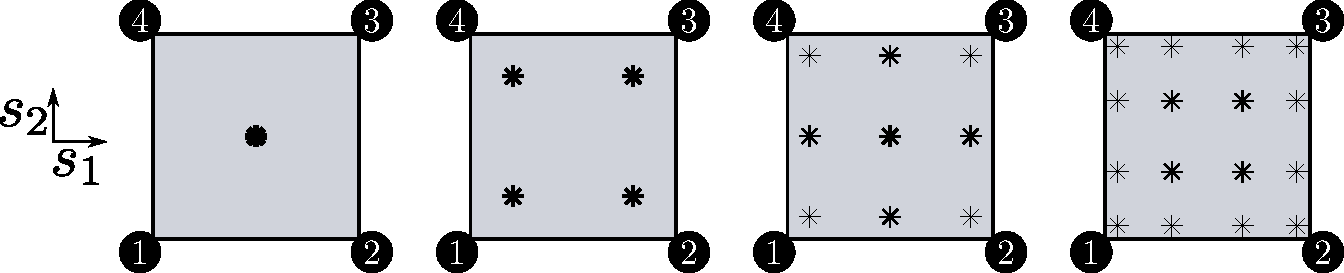
\includegraphics[width=\linewidth]{2d_gaussian_quad.pdf}
    \caption{Examples of 2D Gauss-Legendre quadrature of the parent element with $Q = 1,\, 2,\, 3,\, 4$. The point size represents the weight $w$ of the integration point. The parent elements are centred at the origin and $s_1,\, s_2 \in [-1,\,1]$. We use an anticlockwise node numbering scheme.}
    \label{f:2d_gaussian_quad}
\end{figure}
%        
\begin{figure}[htb]
    \centering
    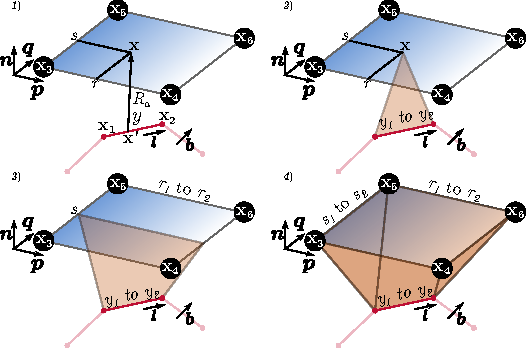
\includegraphics[width=0.8\linewidth]{images/force_calc_linear_rectangle.pdf}
    \caption{Diagram of the parametric line integrals solved by \citet{Queyreau} to find the forces on linear rectangular surface elements.}
    \label{f:force_lin_rect}
\end{figure}
%

\Cref{eq:ddd_fem_force} is actually a triple vector integral. It involves integrating over the surface element and along the dislocation line segment, as shown in \cref{f:force_lin_rect}. Using the isotropic Burgers vector distribution proposed in \cite{Cai2006}, the dyadic form of the stress tensor produced by a straight finite dislocation segment bounded by nodes at $\mathbf{x_1}$ and $\mathbf{x_2}$ is \cite{Queyreau},
%
\begin{align}
    \label{eq:stress}
    \tns{\sigma}(\vec{x}) = &
    - \dfrac{\mu}{8\pi} \int\limits_{\mathbf{x_1}}^{\mathbf{x_2}} \left( \dfrac{2}{R_{a}^{3}} + \dfrac{3a^2}{R_{a}^{5}} \right) \left[ \left(\vec{R} \times \vec{b}\right) \otimes \mathrm{d}\vec{x'} + \mathrm{d}\vec{x'} \otimes \left(\vec{R} \times \vec{b}\right) \right]  \\
    %
                            & + \dfrac{\mu}{4\pi(1-\nu)} \int\limits_{\mathbf{x_1}}^{\mathbf{x_2}} \left( \dfrac{1}{R_{a}^{3}} + \dfrac{3a^2}{R_{a}^{5}} \right) \left[ \left(\vec{R} \times \vec{b}\right) \cdot \mathrm{d}\vec{x'} \right]\vec{I_2}\nonumber                  \\
    %
                            & -\dfrac{\mu}{4\pi(1-\nu)} \int\limits_{\mathbf{x_1}}^{\mathbf{x_2}}  \dfrac{1}{R_{a}^{3}} \left[ \left(\vec{b} \times \mathrm{d}\vec{x'}\right) \otimes \vec{R} + \vec{R} \otimes \left(\vec{b} \times \mathrm{d}\vec{x'}\right) \right]\nonumber \\
    %
                            & + \dfrac{\mu}{4\pi(1-\nu)} \int\limits_{\mathbf{x_1}}^{\mathbf{x_2}} \dfrac{3}{R_{a}^{5}} \left[ \left(\vec{R} \times \vec{b}\right) \cdot \mathrm{d}\vec{x'} \right]\vec{R}\otimes\vec{R}\nonumber,
\end{align}
where
\begin{align}
    \vec{R}            & = \vec{x} - \vec{x'} = y \vec{l} + r \vec{p} + s \vec{q} \\
    %
    R_a                & = \sqrt{\vec{R} \cdot \vec{R} + a^2}                     \\
    %
    \mathrm{d}\vec{x'} & = -\mathrm{d} y \vec{l}
\end{align}
%
The vectors $\vec{p}$ and $\vec{q}$ are aligned with the edges of the rectangular finite element, $\vec{n} = \vec{p} \times \vec{q}$ is the element surface normal (pointing away from the dislocation), and $\vec{l}$ is parallel to the dislocation line segment as shown in \cref{f:force_lin_rect}. Then (provided $\vec{l}$ is not parallel to $\vec{p}$ or $\vec{q}$) $\vec{R}$ can be expressed in terms of $(\vec{l},~\vec{p},~\vec{q})$ with coefficients
%
\begin{align}
    y = \dfrac{\vec{R}\cdot \vec{n}}{\vec{l}\cdot \vec{n}} \label{eq:problem},\quad
    %
    r = \dfrac{\vec{R}\cdot (\vec{q} \times \vec{l})}{\vec{p}\cdot (\vec{q} \times \vec{l})}, \quad
    %
    s = \dfrac{\vec{R}\cdot (\vec{p} \times \vec{l})}{\vec{q}\cdot (\vec{p} \times \vec{l})}\,.
\end{align}
%
Substituting \cref{eq:stress} and \cref{eq:shape_function} into \cref{eq:ddd_fem_force} yields four long and messy equations (one for each FE node) that were elegantly solved by \citet{Queyreau} by utilising the fact that the triple integrals all had the form,
%
\begin{align}
    H_{ijkl}        & = \int\limits_{r_{1}}^{r_{2}}\int\limits_{s_{1}}^{s_{2}}\int\limits_{y_{1}}^{y_{2}} \dfrac{r^i s^j y^k}{R_{a}^{m}}\label{eq:triple_int} \\
    \textrm{when }m & = 5 \textrm{ then } i,\, j \in [0,\,3],~k \in [0,\,2]\nonumber                                                                          \\
    \textrm{when }m & = 3 \textrm{ then } i,\, j \in [0,\,2],~k \in [0,\,1]\nonumber                                                                          \\
    \textrm{when }m & = 1 \textrm{ then } i = j = k = 0\nonumber.
\end{align}
%
Using partial differentiation and integration by parts, they found a series of recurrence relations that lead to double and single integrals with a similar form to equation (\cref{eq:triple_int}). Together they are used to construct a full solution. The recurrence relations stop working when $i = j = k = 0 \textrm{ and } m = 1,\, 3$. At which point, direct integration of the resulting single and double integrals (the last triple integrals all cancel out in the global calculation) yields six seed functions that are used as the starting point for the recurrence relations. Three of them are logarithms and three either arctangents or---if a discriminant is negative---hyperbolic arctangents. The details of the procedure can be found in \cite{Queyreau}.

Although exact, the use of arctangents/hyperbolic arctangents and logarithmic functions, compounded by the large number of recurrence relations is prime territory for error propagation and numerical problems (see \cref{s:method}). This is particularly egregious when using general purpose compilers instead of high-performance or scientific computing compilers where mathematical functions are implemented more precisely. These issues must be taken into account when using analytic tractions in the form of numeric tolerances.

In simulations, the tractions are manifested in the image stresses calculated by the FE solver at FE nodes. In order to validate and compare the practical differences between analytic and gauss quadrature methods, we use them both to calculate the reaction stresses produced by the tractions with the same FE solver and compare the results with the analytic expressions for infinite dislocations in inhomogenous media in \cite{head1953edge} for edge dislocations as well as those for screw dislocations found in \cite[p.~59,~64]{hirth1983theory}, where the traction surface is the line $x=0$, looking at the $xy$-plane in the positive $z$-direction, where the dislocation coordinates are represented by $(a,~c)$ and points in the plane described by their $(x,~y)$ coordinates.

The original paper by \citet{head1953edge} has a few typos that have been replicated in other sources, so we include the complete and correct expressions. \citet{head1953edge} gives two basic cases. The first case in \cref{eq:imageStressAnalyticEdge1} corresponds to the case where $\vec{b}$ is perpendicular to the surface and positive $b$ means it points in the positive $x$ direction,
\begin{subequations}
    \begin{align}\label{eq:imageStressAnalyticEdge1}
        \sigma_{xx} = D (y - c) & \left\{-\dfrac{3 (x - a)^2 + (y - c)^2}{[(x - a)^2 + (y - c)^2]^2} + \dfrac{3 (x + a)^2 + (y - c)^2}{[(x + a)^2 + (y - c)^2]^2}\right.                                             \\\nonumber
                                & \left. + 4 a x \dfrac{3 (x + a)^2 - (y - c)^2}{[(x + a)^2 + (y - c)^2]^3}\right\}\,,                                                                                               \\
        \sigma_{yy} = D (y - c) & \left\{\dfrac{(x - a)^2 - (y - c)^2}{[(x - a)^2 + (y - c)^2]^2} - \dfrac{(x + a)^2 - (y - c)^2}{[(x + a)^2 + (y - c)^2]^2}                                                 \right. \\\nonumber
                                & \left. + 4 a (2 a - x) \dfrac{(x + a)^2 + (3 x + 2 a) (y - c)^2}{[(x + a)^2 + (y - c)^2]^3}\right\}\,,                                                                             \\
        \sigma_{xy} = D         & \left\{(x - a) \dfrac{(x - a)^2 - (y - c)^2}{[(x - a)^2 + (y - c)^2]^2} - (x + a) \dfrac{(x + a)^2 - (y - c)^2}{[(x + a)^2 + (y - c)^2]^2}\right.                                  \\\nonumber
                                & \left. + 2 a \dfrac{6 x (x + a) (y - c)^2 - (x - a) (x + a)^3 - (y - c)^4}{[(x + a)^2 + (y - c)^2]^3}\right\}\,.
    \end{align}
\end{subequations}
The case where the $\vec{b}$ lies parallel to the surface and positive $b$ means it points in the positive $y$ direction, is found in \cref{eq:imageStressAnalyticEdge2},
\begin{subequations}
    \begin{align}\label{eq:imageStressAnalyticEdge2}
        \sigma_{xx} = D         & \left\{ (x - a) \dfrac{(x - a)^2 - (y - c)^2}{[(x - a)^2 + (y - c)^2]^2} -(x + a) \dfrac{(x + a)^2 - (y - c)^2}{[(x + a)^2 + (y - c)^2]^2} \right.     \\\nonumber
                                & \left. + 2 a \dfrac{(3 x + a) (x + a)^3 - 6 x (x + a) (y - c)^2 - (y - c)^4}{[(x + a)^2 + (y - c)^2]^3}\right\}\,,                                     \\
        \sigma_{yy} = D         & \left\{ (x - a) \dfrac{(x - a)^2 + 3 (y - c)^2}{[(x - a)^2 + (y - c)^2]^2} - (x + a) \dfrac{(x + a)^2 + 3 (y - c)^2}{[(x + a)^2 + (y - c)^2]^2}\right. \\\nonumber
                                & \left. - 2 a \dfrac{(x - a) (x + a)^3 - 6 x (x + a) (y - c)^2 + (y - c)^4}{[(x + a)^2 + (y - c)^2]^3}\right\}\,,                                       \\
        \sigma_{xy} = D (y - c) & \left\{\dfrac{(x - a)^2 - (y - c)^2}{[(x - a)^2 + (y - c)^2]^2} - \dfrac{(x + a)^2 - (y - c)^2}{[(x + a)^2 + (y - c)^2]^2} \right.                     \\\nonumber
                                & \left. + 4 a x \dfrac{3 (x + a)^2 - (y - c)^2}{[(x + a)^2 + (y - c)^2]^3}\right\}\,.
    \end{align}
\end{subequations}
Screw dislocations are markedly simpler, as only the shear components are non-zero. Here $\vec{b} = \vec{l}$ and therefore positive $b$ means it points in the positive $z$ direction (away from the observer) \cref{eq:imageStressAnalyticScrew},
\begin{subequations}
    \begin{align}\label{eq:imageStressAnalyticScrew}
        \sigma_{xz} & = -D \left(\dfrac{y - c}{(x - a)^2 + (y - c)^2} - \dfrac{y - c}{(x + a)^2 + (y - c)^2}\right)   \\
        \sigma_{yz} & = D \left(\dfrac{x - a}{(x - a)^2 + (y - c)^2} - \dfrac{x + a}{(x + a)^2 + (y - c)^2}\right)\,.
    \end{align}
\end{subequations}
In every case, the constant $D$ is defined by \cref{eq:Dconstant}
\begin{align}\label{eq:Dconstant}
    D = \dfrac{\mu}{2\pi} \cdot \dfrac{1+\nu}{1-\nu^2} \cdot b\,.
\end{align}
Note the first terms of \cref{eq:imageStressAnalyticEdge1,eq:imageStressAnalyticEdge2,eq:imageStressAnalyticScrew} all correspond to the stress field generated by the dislocation. The following terms are the corrective terms required to make the boundary conditions on the surface equal to zero. Therefore, we can split these equations and only look at the real or corrective terms, which we do in order to only visualise the effect of the different traction calculations. Furthermore \cref{eq:imageStressAnalyticEdge1,eq:imageStressAnalyticEdge2,eq:imageStressAnalyticScrew} are all singular at the dislocation coordinates, our simulation code uses non singular expressions found by \citet{Cai2006}, which smooth out drastic increases in stresses and avoid numerical blow up as we near the dislocation core.

\section{Methodology}\label{s:method}
Numerical integration of tractions can produces unexpected behaviour such as force hot spots and sign inversions as a dislocation approaches a surface. During a large simulation, these effects are hard to spot. \Cref{f:err_basic_cantilever} has a quick example of the relative errors for an idealised system not disimilar to what can be found with in a simple cantilever bending simulation with a single dislocation loop. As expected, the errors decrease as the mesh gets finer.
\begin{figure}
    \centering
    \subfloat[$60 \times 16$ elements ($x \times y$).]
    {
        { 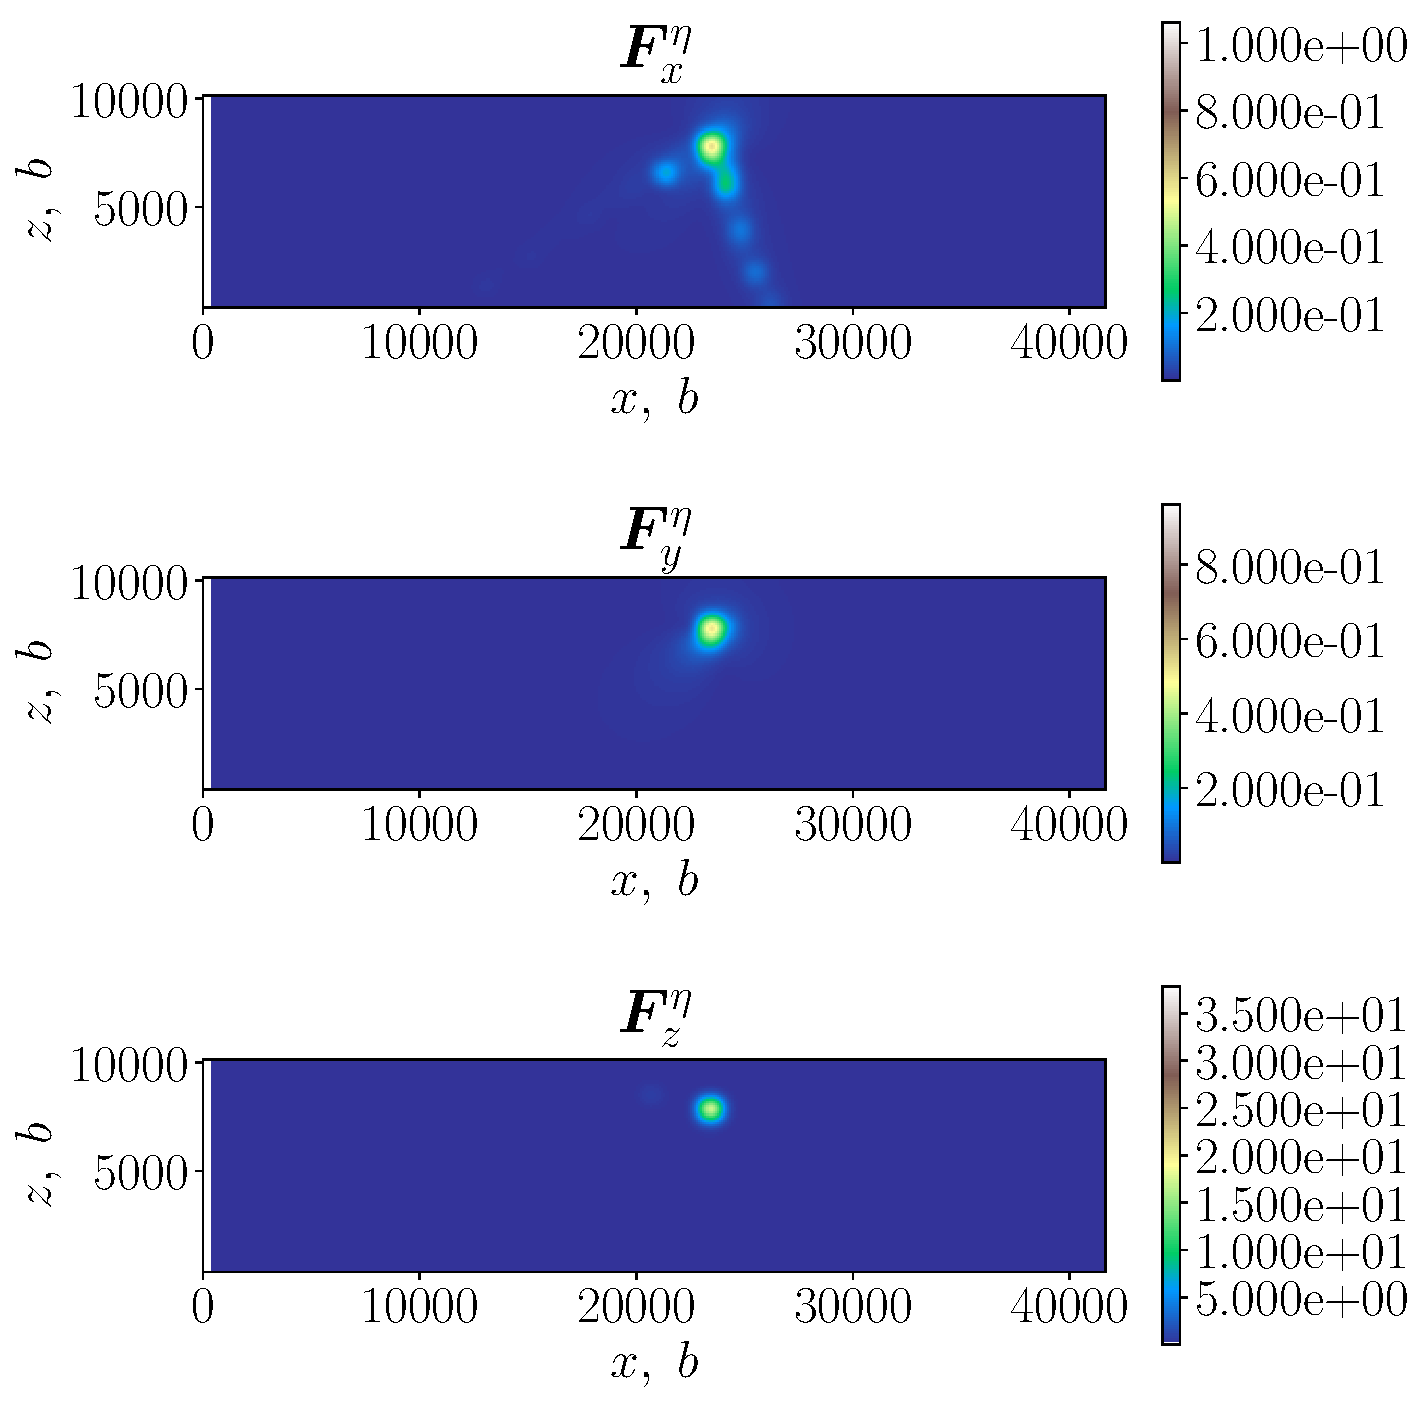
\includegraphics[width=0.45\linewidth]{eta_mx=60_face=1.pdf} }
    }
    ~
    \subfloat[$120 \times 36$ elements ($x \times y$).]
    {
        { 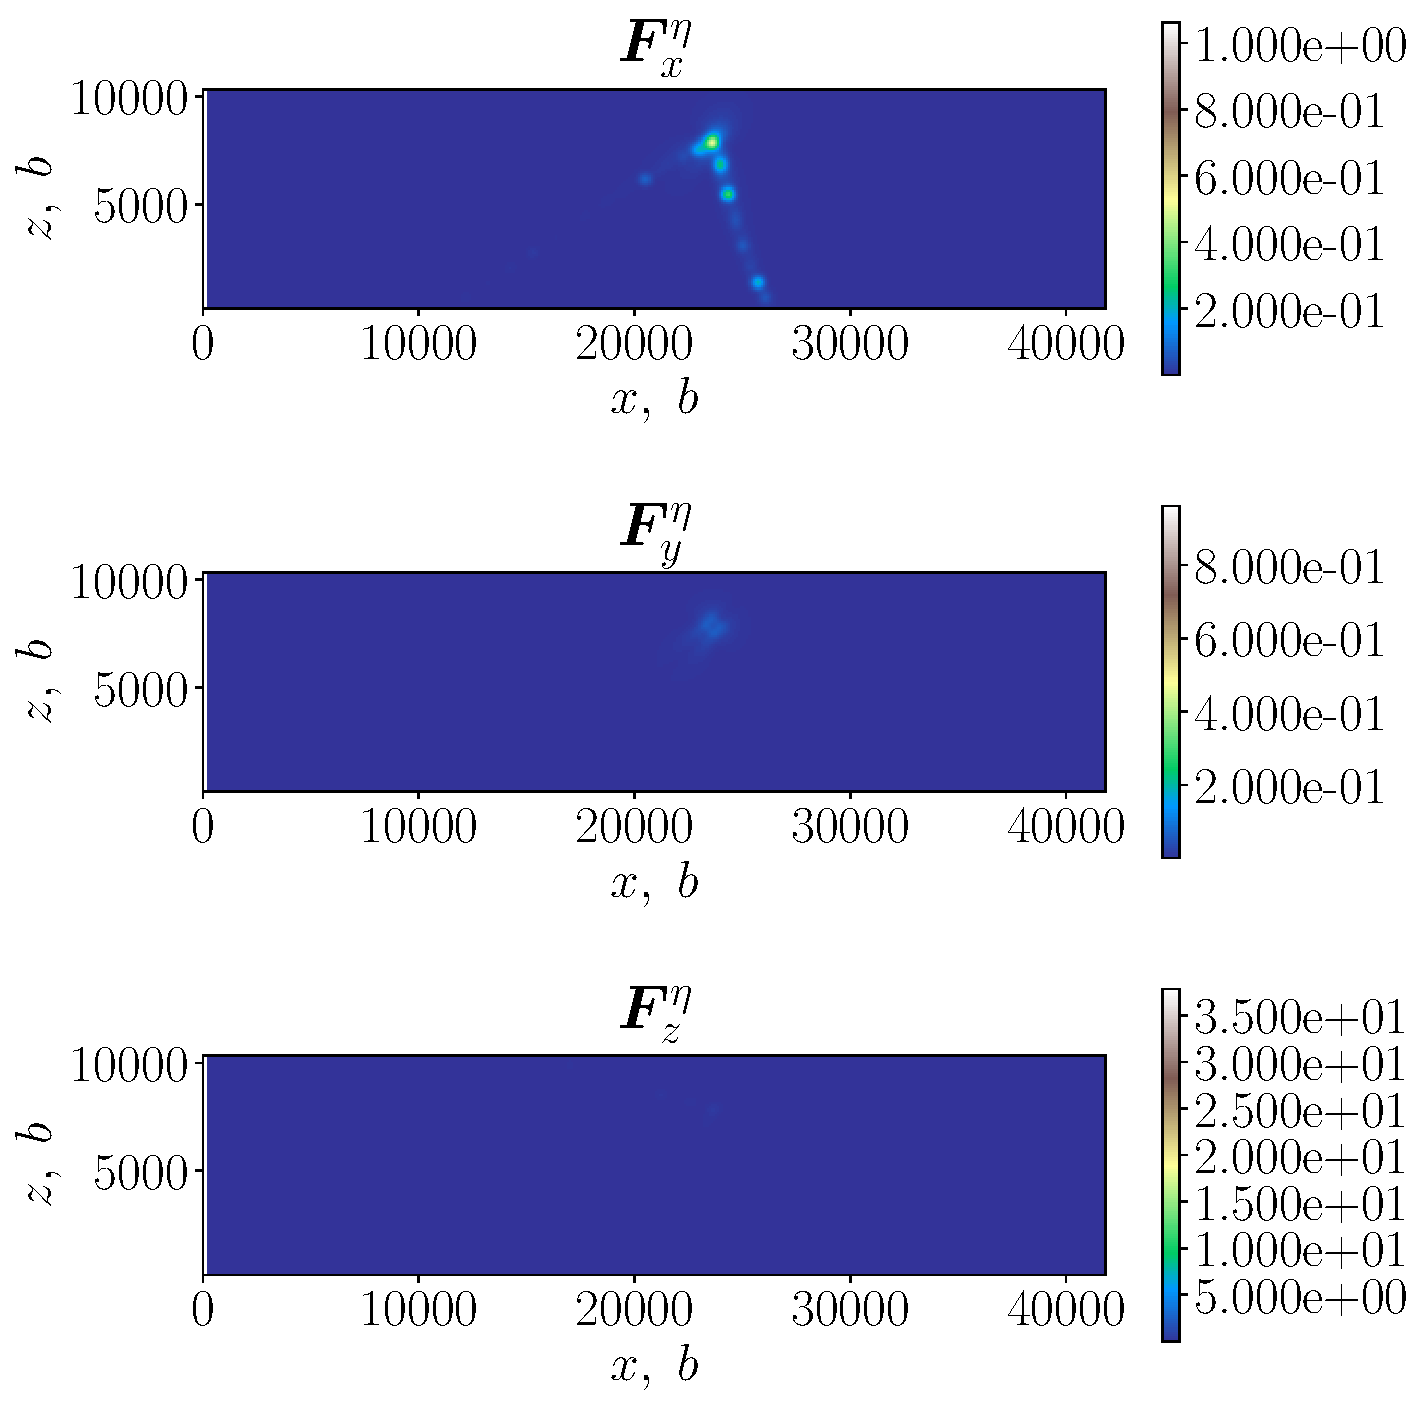
\includegraphics[width=0.45\linewidth]{eta_mx=120_face=1.pdf} }
    }
    \caption{Relative error ($\vec{F}^{\eta}$) in the nodal force obtained using numerical integration with one quadrature point $Q = 1$, and the analytic solution. The $xz$-face of a rectangular cantilever with plane normal, $\vec{n} = \left[0\,\overline{1}\,0\right]$. The dislocation is of pure edge character with $\vec{b} = [1\,0\,\overline{1}]$, and line direction, $\vec{l} = \left[\overline{1}\,2\,\overline{1}\right]/\sqrt{6}$ which pierces both $xz$-faces. The dislocation has its centre at the centroid of the cantilever.}
    \label{f:err_basic_cantilever}
\end{figure}

\citet{Queyreau} identified that for a given number of quadrature points, the error is dependent on the dislocation character but always increases rapidly as the distance between the segment and element surface decrease (see \cref{f:rel_err_perp_edge,f:rel_err_par_edge}).

Expanding the test cases reveals just how problematic numerical integration of the tractions can be when a dislocation approaches a surface. The two basic test cases, an orthogonal and parallel edge segment, are shown in \cref{f:gauss_quad_test}.

The symmetry of the simple test cases can also influence how solution is as the stress fields exhibit symmetries about the dislocation line. If the dislocation is centered at the center of the element and orthogonal to it then the numerical solution becomes more accurate. However isolated test cases are far from typical simulation scenarios. A single quadrature point is often used to evaluate tractions due to the low computational cost and works well for segments which are not close to the surface. This is therefore the benchmark against which we measure the cost-benefit of implementing and utilising the analytic solutions. It should also be noted that by using a single Gauss point, one can use the same FE mesh as for the Gauss points, simplifying the implementation.
%		
\begin{figure}
    \centering
    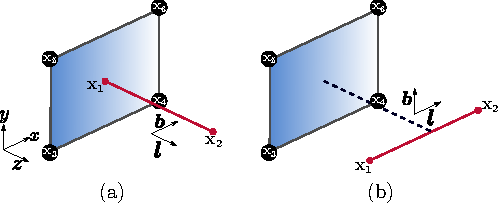
\includegraphics[width=0.8\linewidth]{images/test_gauss_quad.pdf}
    \caption{Simple test cases for an edge segment and surface element perpendicular (a) and parallel (b). The perpendicular dislocation is centered at the midpoint of the surface element, node $\mathbf{x_1}$ is separated by a perpendicular distance $\mathbf{x_1}^z$ to prevent the dislocation from intersecting the surface. On the right, the parallel dislocation runs along the$x$-axis at half the height of the surface element. The nodes of each dislocation line segment are kept at a perpendicular distance of at least one core radius away from the surface element.}
    \label{f:gauss_quad_test}
\end{figure}

\citet{Queyreau} found the analytic solution is approximately 10 times more computationally expensive than its numerical counterpart for 1 quadrature point. The implementation of the analytic solution is also much more involved. One issue is the calculation of the $y$-coordinate in the local coordinate frame as shown in \cref{f:force_lin_rect} and \cref{eq:problem}, if $\vec{l} \perp \vec{n}$, we get a singularity. As mentioned in \cite{Queyreau}, an easy fix is to rotate the line segment about its midpoint around the $\vec{l} \times \vec{n}$ axis and use the mean values either side as the true result. An example of what this looks like in terms of forces can be seen in \cref{f:rotate} (we removed the singularity to keep the graph smooth).
\begin{figure}[htb]
    \centering
    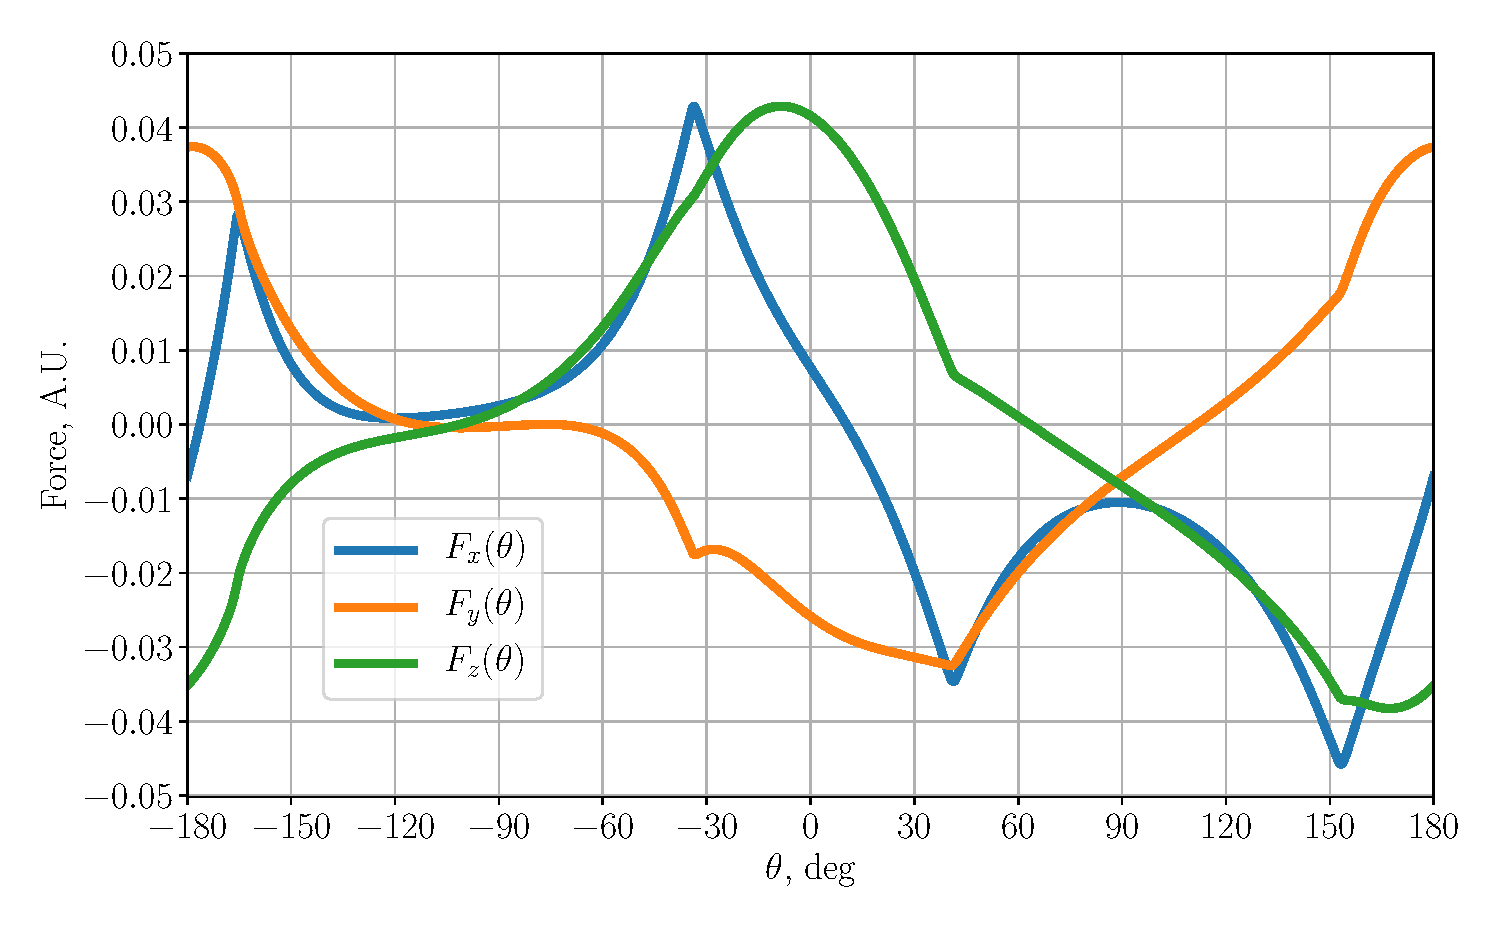
\includegraphics[width=0.8\linewidth]{ftot_rotation_lin_rect.pdf}
    \caption{Example of the components of the total force on a surface element (the force summed over all four FE nodes) as a dislocation segment parallel to the surface element ($\theta = 0$) is rotated about its midpoint around the axis defined by $\vec{l}\times\vec{n}$. The force is smooth but not necessarily antisymmetric about the neighbourhood of $\theta=0$.}
    \label{f:rotate}
\end{figure}
The specific shape of the curves will vary depending on the element-segment configuration, but is smooth and well-behaved about singularity. For our purposes, we used 4 perturbations each of $1\,\deg$, in the clockwise and anti-clockwise directions (8 rotations in total) w.r.t. the parallel position.

However, the check for orthogonality is dependent on the length scales involved in the simulation, we found that machine precision plays an important part in deciding how strict the tolerance should be. If,
%
\begin{align}
    \lvert\vec{l}\cdot\vec{n}\rvert \lesssim \dfrac{\max\left(\lvert\vec{R}\cdot\vec{n}\rvert\right)}{10^8}\,,
\end{align}
%
it is advisable to treat the segment as parallel to the surface element. In our case the numerator on the RHS is simply the cantilever's largest dimension. $10^8$ is used instead of actual machine precision $\sim10^{15}$ because the seed functions and large number of recurrence relations of the solution propagate errors. Smaller tolerances lead to these errors growing so much that the simulation can be impacted; this is a problem when such dislocations move slightly during a simulation and become nearly parallel with the surface, which are detected if the tolerance is too small, yet the limited numerical precision leads to round off and truncation errors during the calculation. Ironically tolerances which are too large can cause the perturbations to rotate the dislocation segment closer to the singularity also producing erroneous results. Larger than necessary tolerances can also slow down the calculation by detecting dislocations that are far enough from the special case that they can be treated like non-parallel segments.

In general one does not want a dislocation segment to intersect the surface when it is being rotated. Naively one would calculate the maximum rotational angle, $\theta_{\textrm{max}}$, to be,
%
\begin{align}
    \theta_{\textrm{max}} & = \arctan\left(\dfrac{2 d}{\left\lvert\mathbf{x_2} - \mathbf{x_1}\right\rvert}\right)\,,
\end{align}
%
where $d$ is the minimum orthogonal distance from the dislocation to the surface element (collision distance), and $\mathbf{x_1},\,\mathbf{x_2}$ are the dislocation segment node coordinates. However, $\theta_\textrm{max}$ might be too small (due to numerical precision) in cases when the segment length is too small compared to the distance to a surface element or when the segment length is much greater than $d$. Fine tuning the angle is a task that involves knowing the minimum collision distance, minimum segment length, dislocation core radius, and the compiler's implementation of mathematical functions. Given the rarity of such cases and their comparatively low impact, we chose our perturbation such that we safely avoid this problem.

Furthermore, the chirality and self-consistency of the  FE nodes must be accounted for such that they are in the proper order regardless of the element face they belong to. Here we use 8  node linear hexahedral (brick) elements with the node numbering shown in \cref{f:fe_numbering}. The node ordering for the various surfaces are obtained by placing an observer inside the element and noting the nodes for the faces of the element, these are shown in \cref{f:surface_nodes}.
%
\begin{figure}
    \centering
    \subfloat[Node numbering for our FE voxels.\label{f:fe_numbering}]
    {
        { 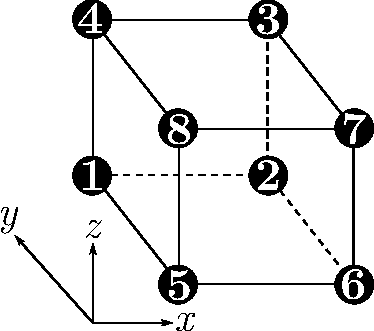
\includegraphics[width=0.375\linewidth]{images/fe_numbering.pdf} }
    }
    \hfill
    \subfloat[Surface nodes selected for each face.\label{f:surface_nodes}]
    {
        { 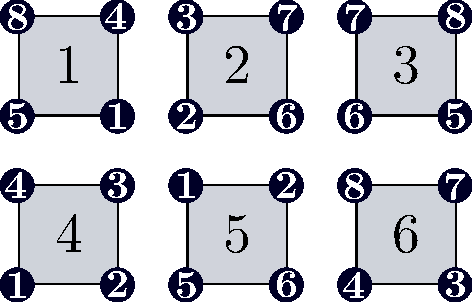
\includegraphics[width=0.525\linewidth]{images/surf_node_plane.pdf} }
    }
    \caption{Surface element nodes must be self-consistent so the forces have the correct sign.}
\end{figure}
%
The total force on a given node must include the force contributions from every element in which said node appears, see \cref{f:shared_node}.
%
\begin{figure}[htb]
    \centering
    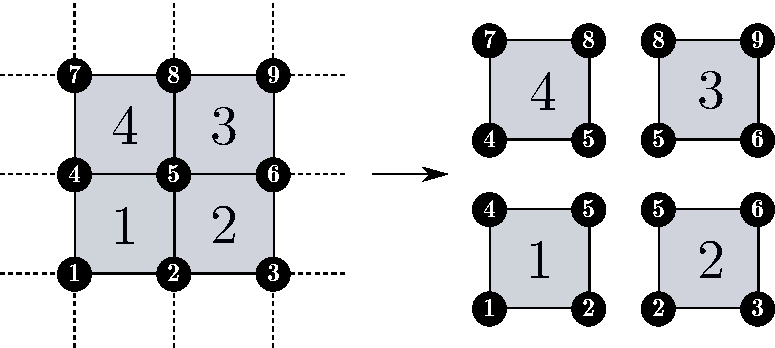
\includegraphics[width=\linewidth]{images/lrse_thread_map.pdf}
    \caption{FE nodes are shared by either 4 element faces or 3 if it is a corner node. The total force on a given node is the summation of the force contributions from each element it belongs to.}
    \label{f:shared_node}
\end{figure}
%
The specifics of the mapping depend on the global FE node numbering. Using \cref{f:shared_node} as our reference labels for elements and nodes, $e$ and $n$ respectively, we can give a concrete example of how this is done by defining,
\begin{subequations}
    \begin{align}
        \vec{x_{e,n}} & \equiv	\begin{bmatrix}
            x_{e,n} & y_{e,n} & z_{e,n}
        \end{bmatrix}^{\mathsf{T}}, \quad
        \vec{x_{n}} \equiv	\begin{bmatrix}
            x_{n} & y_{n} & z_{n}
        \end{bmatrix}^{\mathsf{T}}            \\
        \begin{split}
            \mtx{N_{L}} &=	\begin{bmatrix}
                l_{1,1} & l_{1,2} & l_{1,4} & l_{1,5} \\
                l_{2,2} & l_{2,3} & l_{2,5} & l_{2,6} \\
                l_{3,5} & l_{3,6} & l_{3,8} & l_{3,9} \\
                l_{4,4} & l_{4,5} & l_{4,7} & l_{4,8} \\
            \end{bmatrix}
        \end{split}
        , \quad
        \vec{\gamma} =   \begin{bmatrix}
            l_1    \\
            l_2    \\
            \vdots \\
            l_9
        \end{bmatrix}                          \\
        \begin{split}
            \mtx{F_{e}} &=	\begin{bmatrix}
                \vec{x_{1,1}} & \vec{x_{1,2}} & \vec{x_{1,4}} & \vec{x_{1,5}} \\
                \vec{x_{2,2}} & \vec{x_{2,3}} & \vec{x_{2,5}} & \vec{x_{2,6}} \\
                \vec{x_{3,5}} & \vec{x_{3,6}} & \vec{x_{3,8}} & \vec{x_{3,9}} \\
                \vec{x_{4,4}} & \vec{x_{4,5}} & \vec{x_{4,7}} & \vec{x_{4,8}} \\
            \end{bmatrix}
        \end{split}
        ,\quad
        \vec{\tilde{F}} = 	\begin{bmatrix}
            \vec{x_{1}} \\
            \vec{x_{2}} \\
            \vdots      \\
            \vec{x_{9}}
        \end{bmatrix}\,.\label{eq:force_imp}
    \end{align}
\end{subequations}
Where $\vec{x_{e,n}}$ is a $3\times1$ column vector corresponding to the $x,~y,~z$ dislocation induced forces on node $n$ on the surface element $e$. There are four of these per rectangular surface element, where a given node, $n$, can appear in multiple surface elements (e.g. node 5 in \cref{f:shared_node} is shared by all 4 surface elements), all of which independently contribute to the total force on said node. $\vec{x_n}$ is a $3\times1$ column vector corresponding to the total $x,~y,~z$ dislocation induced forces on node $n$. These are used to shorten the definition of \cref{eq:force_imp} and are not explicitly defined in the implementation, rather they give the force matrices $\mtx{F_{e}}$ and $\vec{\tilde{F}}$ a specific row order. $\mtx{N_{L}}$ is crucial for the correct implementation of this analytical solution in traditional FE codes. It is the $E\times4$ matrix corresponding to the global label of each node in a given surface element. Each row of the matrix represents a surface element and each column represents a node in the surface element. We cannot na\"ively add the columns together as that would give the total force acting on the element as a whole, not each FE node individually. We chose to arrange the columns in accordance to \cref{f:force_lin_rect} as it makes it easier to implement the solution, but the only thing that matters is that the basis vectors $\vec{n},\,\vec{p},\,\vec{q}$ are calculated appropriately. $\vec{\gamma}$ is the vector with the FE node labels, which makes mapping force to node possible. $\mtx{F_{e}}$ is the $3E \times 4$ matrix where the forces acting on each of the four nodes (column) in a particular surface element (each element corresponds to three consecutive rows because there are three dimensions) are stored. $\vec{\tilde{F}}$ is the $3N\times1$ column vector where the total forces on each node are stored (each node has three rows because there are three dimensions). This is easily generalisable to $E$ elements and $N$ nodes.

The following algorithm illustrates how the total force on each node is obtained. The resulting force vector is later used in \cref{eq:thatbc} as $\tilde{\vec{T}} \equiv \tilde{\vec{F}}$.
\begin{algorithm}
    \caption{Assuming $ \vec{\tilde{F}} $ is arranged the same way as $ \vec{\gamma} $ and indexing starts at 0.}
    \begin{algorithmic}[1]
        \label{a:tot_force}
        \State\Comment{Loop through the array containing the node labels of the relevant surface nodes.}
        \For{$ i = 0;\, i < \rvar{length}(\vec{\gamma});\, i++$}					\State\Comment{Save the global node label for the current iteration.}
        \State $ n \gets \vec{\gamma}[i] $
        \State\Comment{Use the node label to find a vector, $\vec{L}$, with the linearised indices in $\mtx{N_{L}}$ where node $n$ appears as part of a surface element whose tractions we are calculating.}
        \State $ \vec{L} \gets \rvar{find}(\mtx{N_{L}} == n) $
        \State\Comment{Loop over coordinates.}
        \For{$ k = 0;\, k < 3;\, k++ $}
        \State\Comment{Use global node label vector to index the force array from the analytical force calculation. Multiplied by 3 because there are three coordinates per node. We sum the forces from the analytical calculation because the same global node can be part of multiple surface elements. We add $ k $ because the $ x,~y,~z $ coordinates are consecutively stored in $ \mtx{F_{e}} $.}
        \State $ \vec{\tilde{F}}[3n + k] \gets \vec{\tilde{F}}[3n + k] + \sum\mtx{F_{e}}[3\vec{L} + k]  $
        \EndFor
        \EndFor
    \end{algorithmic}
\end{algorithm}
Our implementation does not strictly follow \cref{a:tot_force} because we memoise a generalised version of $\vec{L}$ upon simulation initialisation instead of finding one at every iteration, reducing computational time but requiring us to account for nodes without traction boundary conditions. Our indexing also starts at 1, but zero indexing makes the algorithm easier to follow.

After the tractions have been calculated, they are used by the FE solver to generate the corresponding image stresses. \Cref{f:headvstractionfem} shows the system we used to compare the image stresses calculated by our FE solver using numeric tractions v.s. analytic tractions v.s. infinite-domain, singular image stresses found in \cref{eq:imageStressAnalyticEdge1,eq:imageStressAnalyticEdge2,eq:imageStressAnalyticScrew}. We use three test cases, two edge dislocations and one screw, all of which have line direction $\vec{l} = [0\, 0\, 1]$ with Burgers vectors $\vec{b}_\textrm{e1} \equiv \vec{b} = [1\, 0\, 0]$, $\vec{b}_\textrm{e2} \equiv \vec{b} = [0\, 1\, 0]$ \cite{head1953edge}, and $\vec{b}_\textrm{s} \equiv \vec{b} = \vec{l} = [0\, 0\, 1] $ \cite{hirth1983theory}.
\begin{figure}
    \centering
    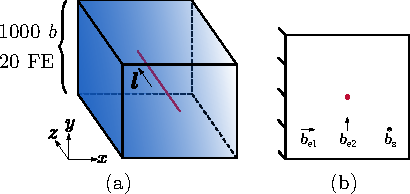
\includegraphics[width=0.8\linewidth]{head_vs_fe_tractions_setup_diagram.pdf}
    \caption{Dislocation parallel to a surface described by the line $x = 0$ (the $yz$-plane in 3D), where the dislocation coordinates are $(a,~c)$, looking down the $xy$-plane where the $x$-axis is horizontal and the $y$-axis vertical. (a) describes the box we used for our comparison, a  $20 \times 20 \times 20$ element cubic box with side lengths equal to $1000~ \lVert \vec{b} \rVert$ with $\vec{T} = \vec{0}$ traction boundary conditions only on the nodes occupying the $yz$-plane and $\vec{U} = \vec{0}$ displacement conditions everywhere else, and a dislocation with line direction in the positive $z$ direction. (b) is the 2D view with the dislocation coordinates $(a,~c)$, as well as the two edge Burgers vectors as described by \cite{head1953edge}, $\vec{b}_\textrm{e1} \equiv \vec{b} = [1\, 0\, 0]$, $\vec{b}_\textrm{e2} \equiv \vec{b} = [0\, 1\, 0]$ and the screw Burgers vector $\vec{b}_\textrm{s} \equiv \vec{b} = \vec{l} = [0\, 0\, 1] $ as posited in \cite{hirth1983theory}.}
    \label{f:headvstractionfem}
\end{figure}

% TODO #48
Finally, we ran a simple simulation where the differences between methods can be readily observed.

\section{Results}\label{s:results}

Isolated test cases were useful in order to gain insight into the differences between the numerical and analytical approaches. When the stress field on the surface element is highly symmetric, numerical integration works well; showing good convergence with increasing number of quadrature points.

\Cref{f:rel_err_perp_edge} shows that even for dislocations only one dislocation core radius ($5b$) away from the surface element, the force can be obtained, up to numerical precision, with 1000 Gauss quadrature points $Q$, for all segment lengths tested. It also shows a very peculiar issue Gauss quadrature has when computing integrals of rational functions when the Gauss points are close poles/maximal values. This undesirable behaviour is observed in the case where $Q = 11$. Where the highest weighted Gauss node is closest to the point where $1/R_{a}$ is maximal, resulting in lower accuracy when compared to $Q = 2, 10$ in \cref{f:rel_err_perp_edge} (a) and (b).
\begin{figure}
    \centering
    \subfloat[Segment starts a single dislocation core radius away.]
    {
        {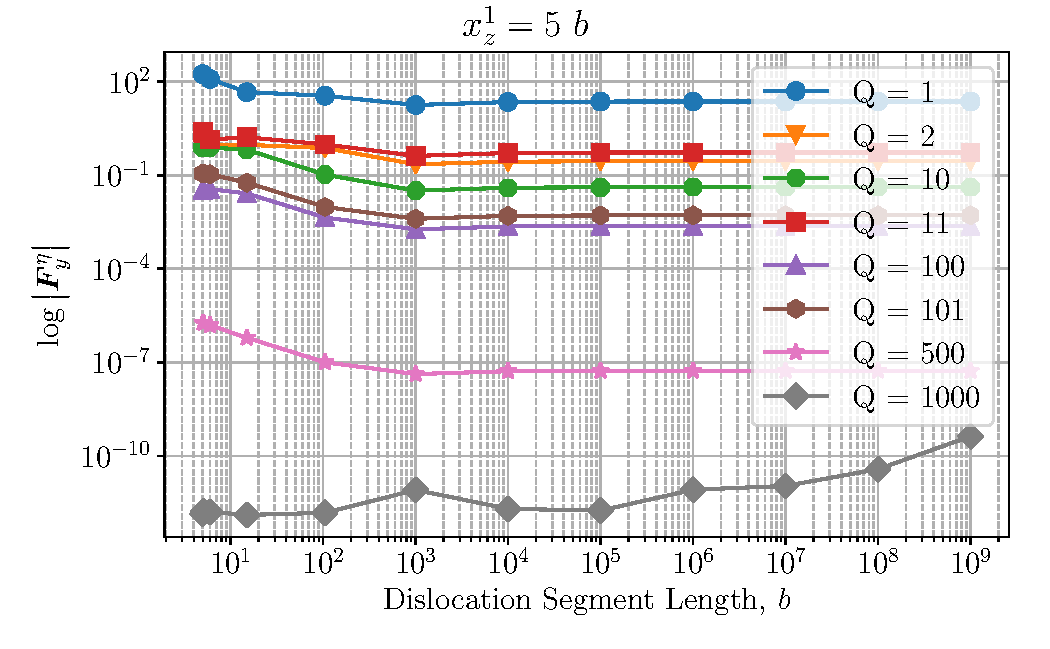
\includegraphics[trim={0.5cm 0.55cm 0.65cm 0.1cm},clip,width=0.475\linewidth]{perp_e_xz=5.pdf}}
    }
    ~
    \subfloat[Segment starts 3 dislocation core radii away.]
    {
        {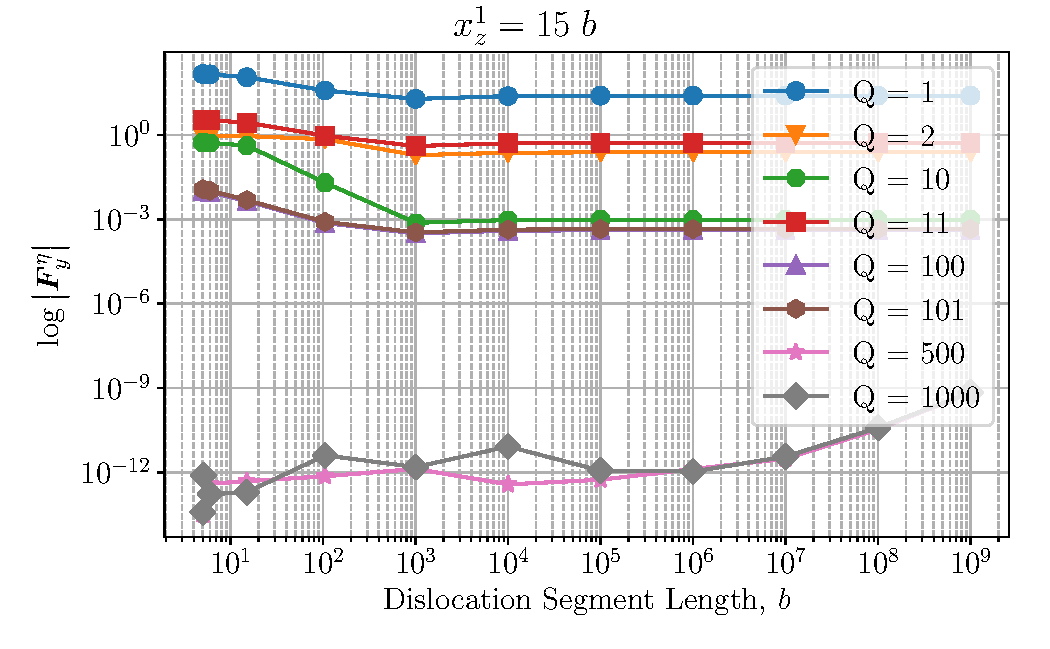
\includegraphics[trim={0.5cm 0.55cm 0.65cm 0.1cm},clip,width=0.475\linewidth]{perp_e_xz=15.pdf}}
    }

    \subfloat[Segment starts 201 dislocation core radii away.]
    {
        {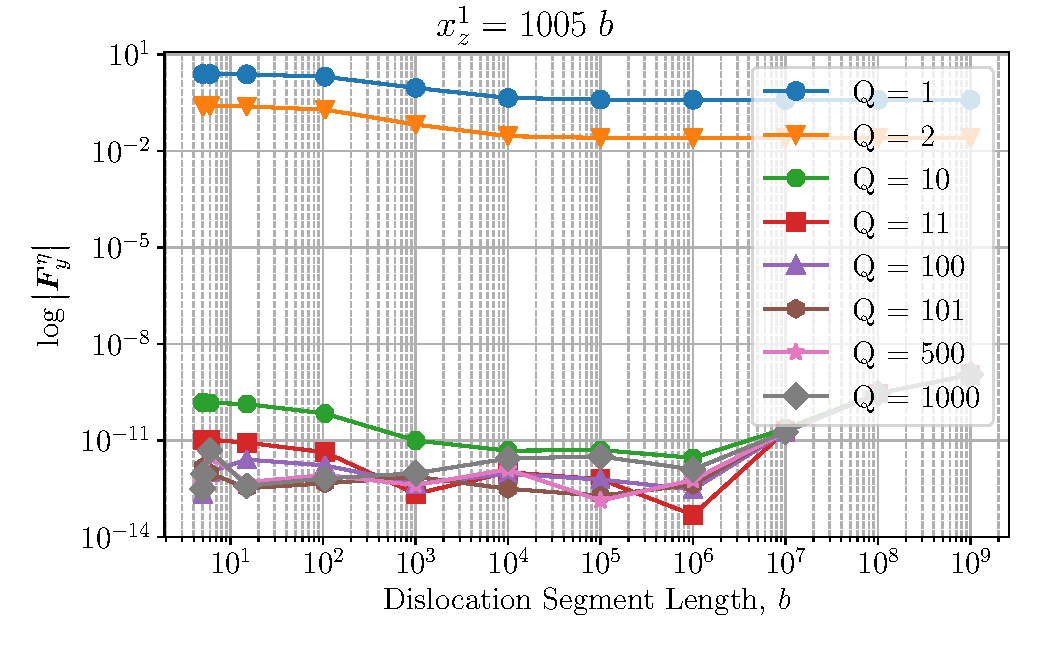
\includegraphics[trim={0.5cm 0.55cm 0.65cm 0.1cm},clip,width=0.475\linewidth]{perp_e_xz=1005.pdf}}
    }
    ~
    \subfloat[Segment starts 20001 dislocation core radii away.]
    {
        {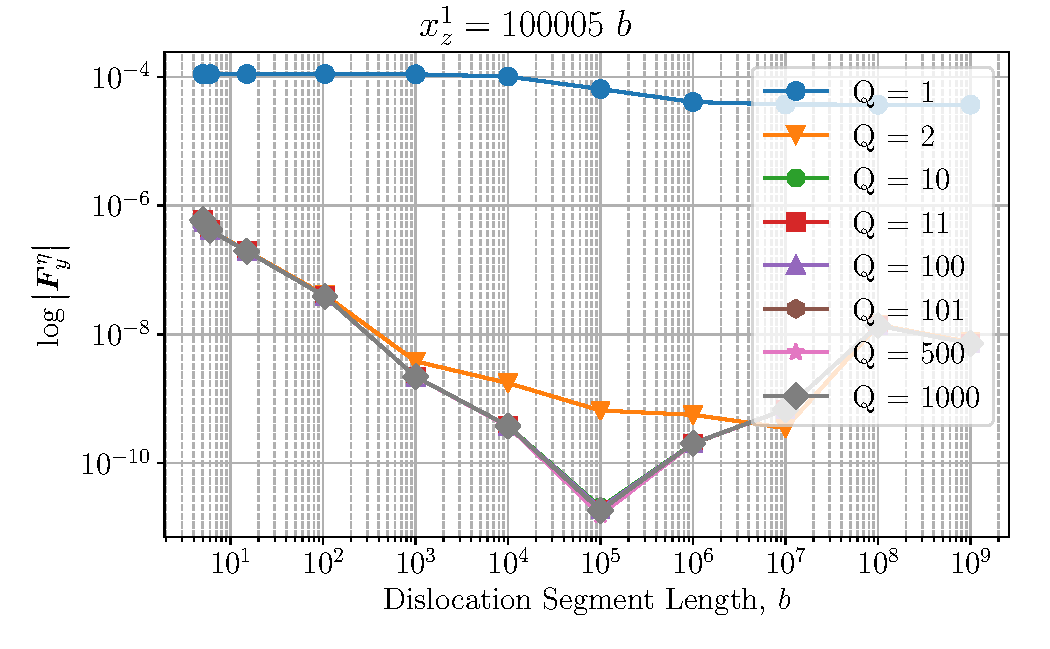
\includegraphics[trim={0.5cm 0.55cm 0.65cm 0.1cm},clip,width=0.47\linewidth]{perp_e_xz=100005.pdf}}
    }
    \caption{Log-log plot of the relative error as a function of dislocation segment length for a perpendicular edge dislocation (\cref{f:gauss_quad_test}a). $x^{1}_{z}$ is the $z$-coordinate of node $\mathbf{x_1}$. $\vec{b} = [1 0 0]$, line direction, $\vec{l} = [0 0 1]$, and dislocation core radius, $a = 5b$, the surface element's normal and size are, $\vec{n} = [0 0 1]$, $L = 1000b$, respectively. $Q$ is the number of quadrature points per dimension.}
    \label{f:rel_err_perp_edge}
\end{figure}

The limitations of Gauss quadrature become even more evident when the dislocation line segment is parallel to a surface element. \Cref{f:rel_err_par_edge} shows the relative errors for a parallel edge dislocation.
\begin{figure}
    \centering
    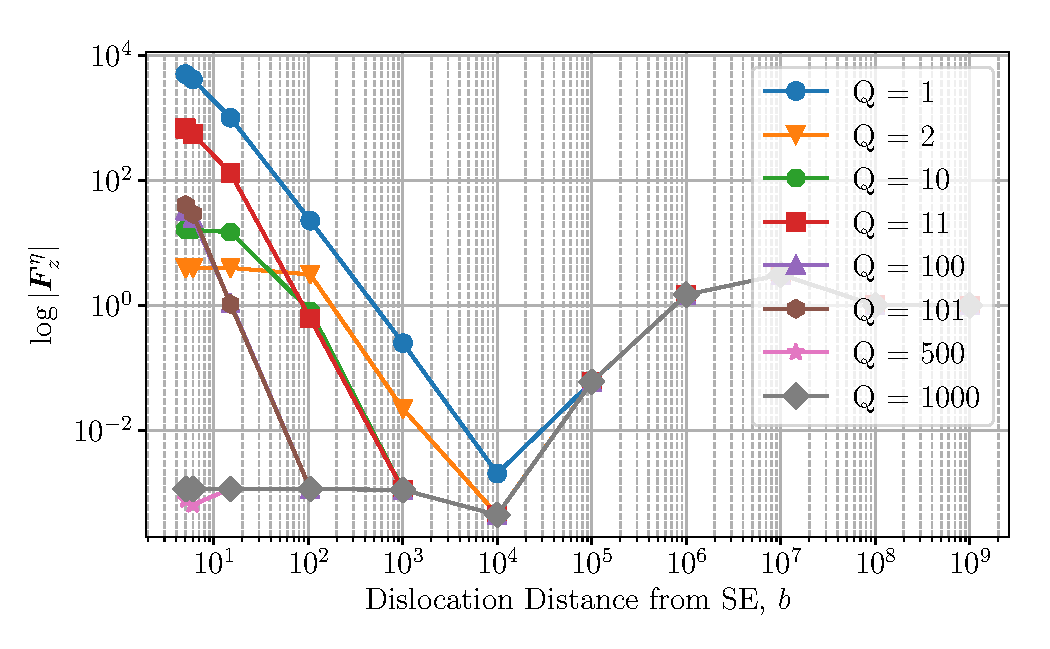
\includegraphics[width=0.8\linewidth]{par_e_z.pdf}
    \caption{Log-log plot of the relative error as a function of distance from the surface element for a parallel edge dislocation (\cref{f:gauss_quad_test}b). Burgers vector, $\vec{b} = [0 1 0]$, line direction, $\vec{l} = [1 0 0]$, dislocation core and surface element parameters are the same as \cref{f:rel_err_perp_edge}. The dislocation length is fixed to $10^{6}\, b,\, x\in\left[-0.5\times10^{6},\, 0.5\times10^{6} \right]$ and bisects the surface element along the $[1 0 0]$ direction. The whole dislocation was segmented into $10^4$ pieces of length $100\, b$ to prevent the dislocation from intersecting the surface element when they were rotated to avoid the singularity. The relative error at large distances ($>10^6 b$) converges to one due to artifacting when dividing two very small double precision numbers. The absolute error always goes towards zero with increasing distance from the surface.}
    \label{f:rel_err_par_edge}
\end{figure}
In \cref{f:rel_err_par_edge}, we observe the relative errors decrease and then converge to $\sim 1$ as the distance grows larger. The convergence to $\sim 1$ is an artifact arising from the fact that the forces on the surface element get asymptotically closer to zero with increasing distance from the surface element, resulting in the division of two increasingly similar, small, non-zero numbers, resulting in $\sim 1$ when done with limited precision. Given infinite precision, it is not unreasonable to assume the relative error would converge to $\sim10^{-3},~ \sim10^{-4}$\footnote[1]{The absolute error \textit{always} decreases as the distance from the surface element increases, but absolute errors are not as useful tools of comparison as long as we are conscious of small artifacting from limited precision.}. However, when the segment is close to the surface, the relative errors are large ($\gg1$) unless using a large number of quadrature points, for example \cref{f:gauss_quad_test}(a) shows that $Q\geq100$ are required when the distance $x^1_z = 15b$. This figure backs up the earlier point regarding Gauss nodes close to maximal rational values, as $Q = 2$ performs significantly better than $Q = 10, 11, 100, 100$ at smaller distances from the surface. Generally, there is no best value of $Q$ other than very large.

From \cref{f:rel_err_perp_edge,f:rel_err_par_edge} one might be tempted to say that for a segment parallel to a surface, Gauss quadrature performs far worse than for a perpendicular one. However there is a further wrinkle in this problem: symmetry. To exemplify this we plot the relevant components of the stress tensor for the arrangement in \cref{f:gauss_quad_test}(a) we find \cref{f:sigma_perp_edge}. The $\sigma_{xz}$ and $\sigma_{zz}$ components are antisymmetric about the centre of the element. If we use Gauss quadrature on them, we sample equivalent but oppositely valued points that equally weighted, thus the sum vanishes. $\sigma_{yz}$ does not, but it can be accurately integrated with sufficiently large $Q$. If we were to move the dislocation off-centre such that the rotational anti-symmetry about the origin is broken, the errors would increase.

\begin{figure}
    \centering
    \subfloat[$\sigma_{xz}$.\label{sf:xzeperp}]
    {
        {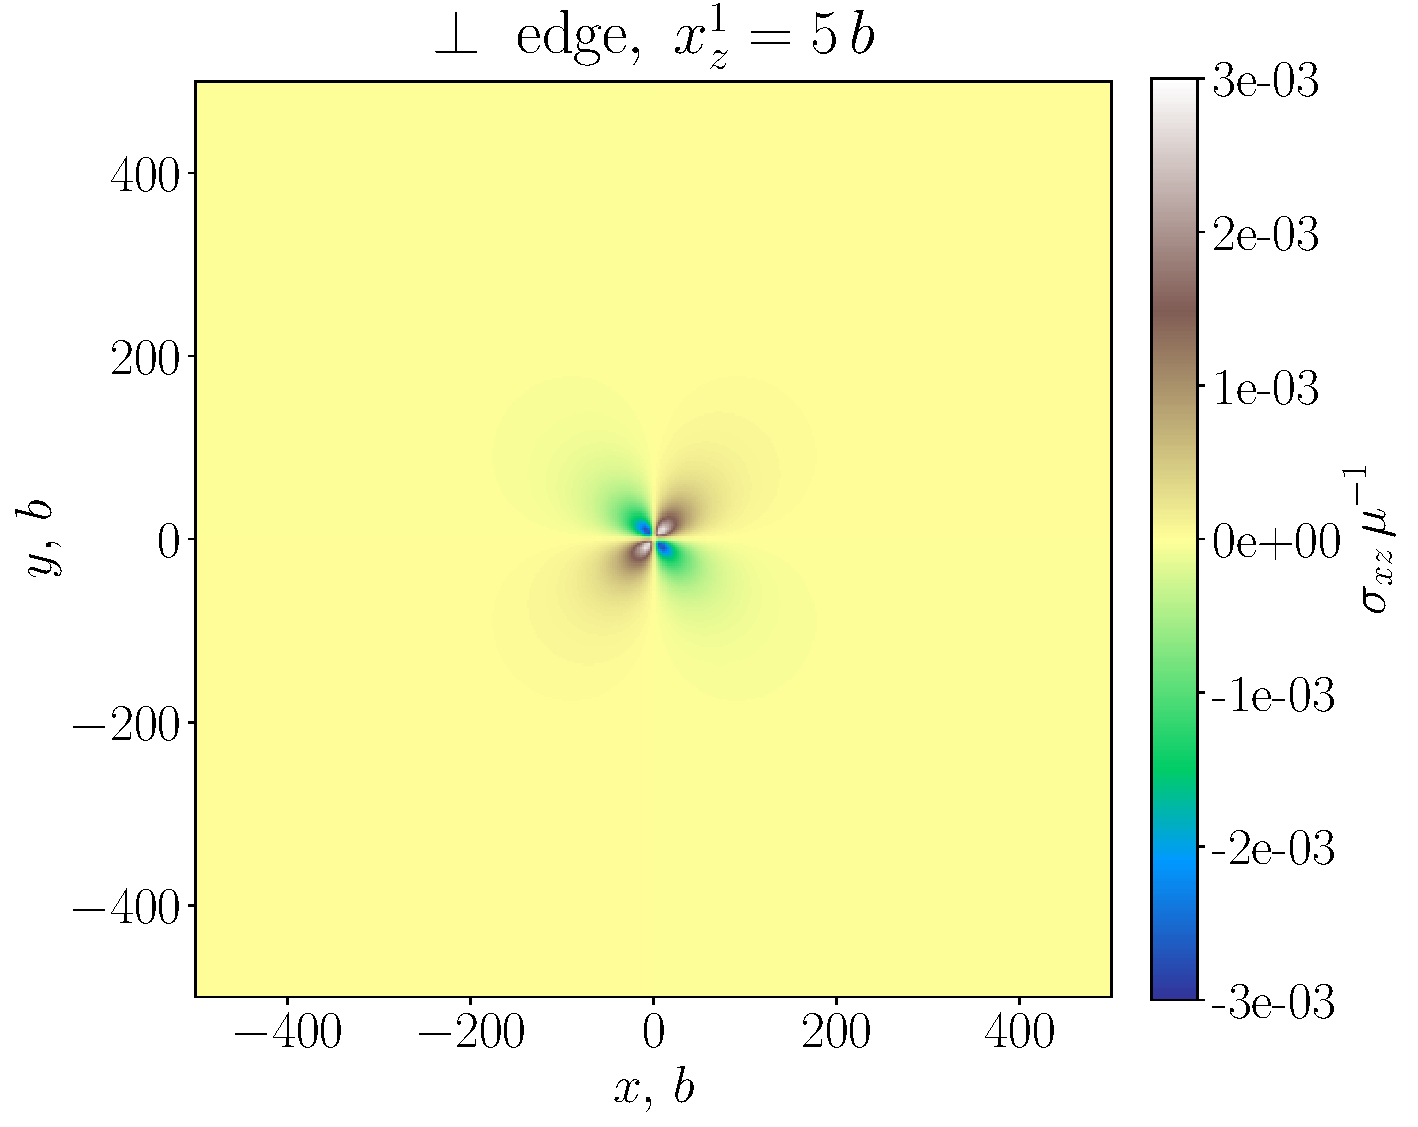
\includegraphics[width=0.3\linewidth]{images/xz_eperp_5_000000.pdf}}
    }
    ~
    \subfloat[$\sigma_{yz}$.\label{sf:yzeperp}]
    {
        {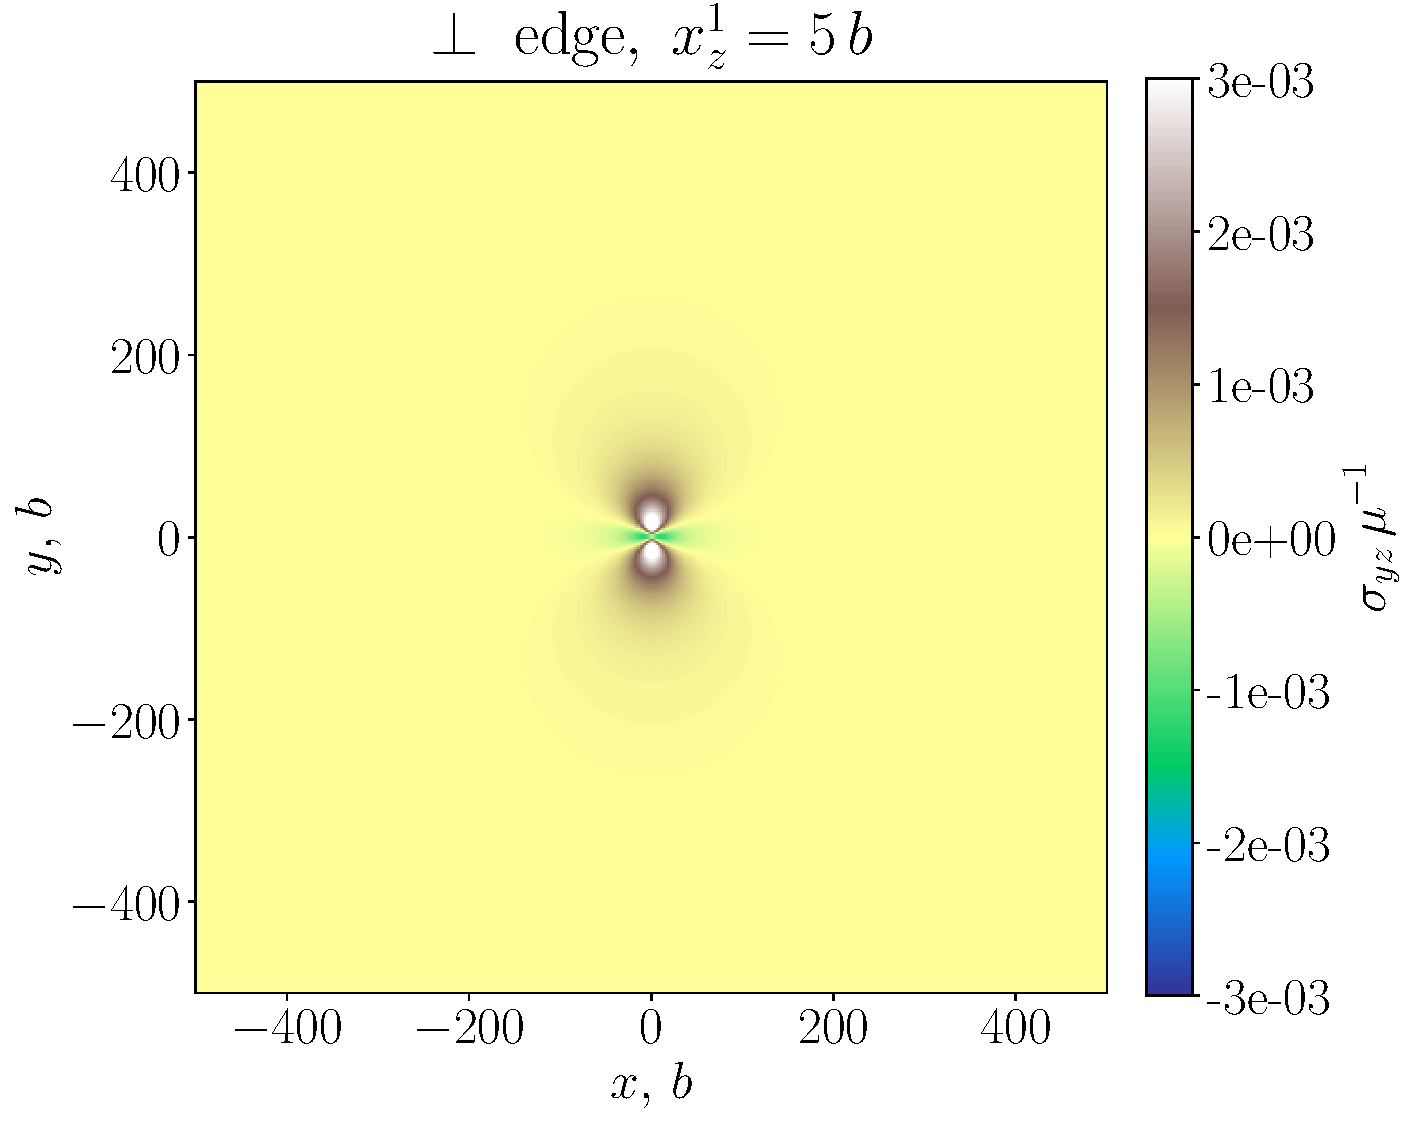
\includegraphics[width=0.3\linewidth]{images/yz_eperp_5_000000.pdf}}
    }
    ~
    \subfloat[$\sigma_{zz}$.\label{sf:zzeperp}]
    {
        {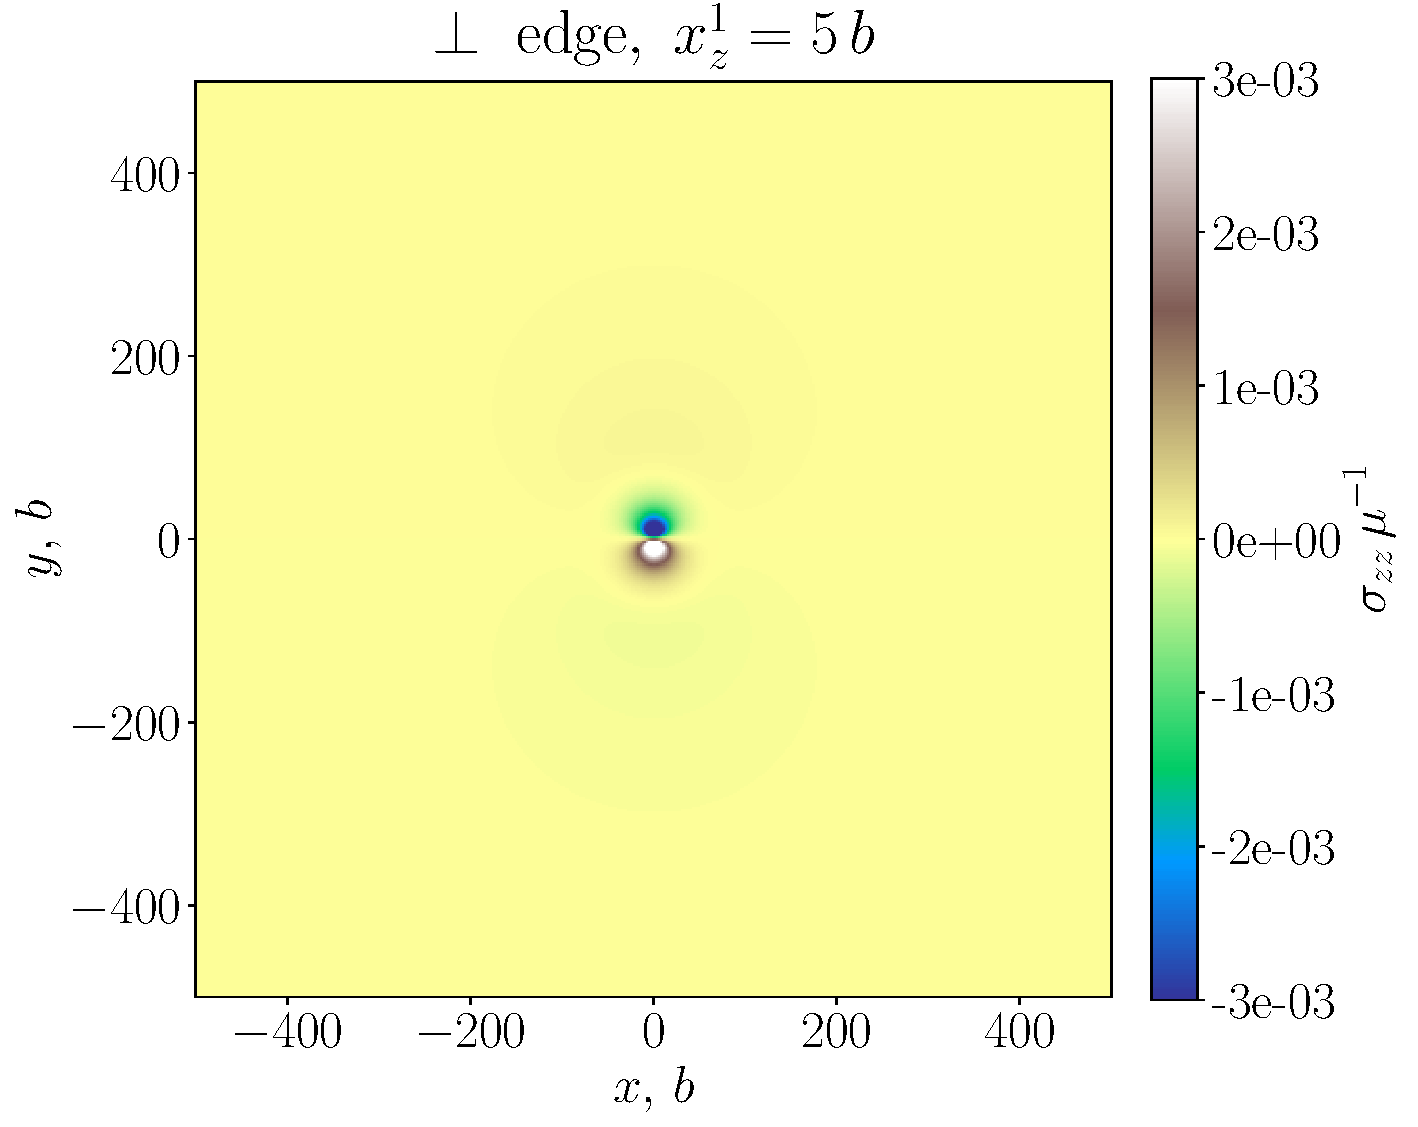
\includegraphics[width=0.3\linewidth]{images/zz_eperp_5_000000.pdf}}
    }
    \caption{Relevant stress components to \cref{f:rel_err_perp_edge}. The antisymmetry of $\sigma_{xz}$ and $\sigma_{zz}$ makes them vanish when integrating. $\sigma_{yz}$ does not vanish, but its symmetry means Gauss quadrature works if sufficient quadrature points are used.}
    \label{f:sigma_perp_edge}
\end{figure}

Despite these being somewhat contrived examples that illustrate the failings of Gauss quadrature, problematic scenarios are commonly to show up in simulations. They are worse with smaller core radii $a$, fewer Gauss nodes, higher dislocation densities near surfaces and more permissive mobility functions. They are fairly localised given the $\mathcal{O}(1/R)$ decay but under unfortunate cirumstances, these spikes in the image forces result in unwarranted topological changes to the dislocation structure by causing segments to move in erroneous or erratic ways. Such changes to the dislocation structure tend to have large and cascading effects as simulations advance. Which is particularly deleterious when doing simulations with higher dislocation densities and/or where a large number of dislocations are close to the surface, such as nanoindentation simulations.

As stated in \cref{s:method}, tractions are used to calculate the image stresses resulting from the boundary conditions. We therefore also compare the differences in image stresses resulting from numeric ($Q = 1$) and analytic traction calculations and how they compare to the infinite-domain, singular expressions in \cref{eq:imageStressAnalyticEdge1,eq:imageStressAnalyticEdge2,eq:imageStressAnalyticScrew}\footnote{The first term in each equation corresponds to the real stresses, we can omit these to view the image stresses.}.

\begin{figure}
    \centering
    \subfloat[$\hat{\sigma}_{xx}$.\label{sf:sxxeperp}]
    {
        {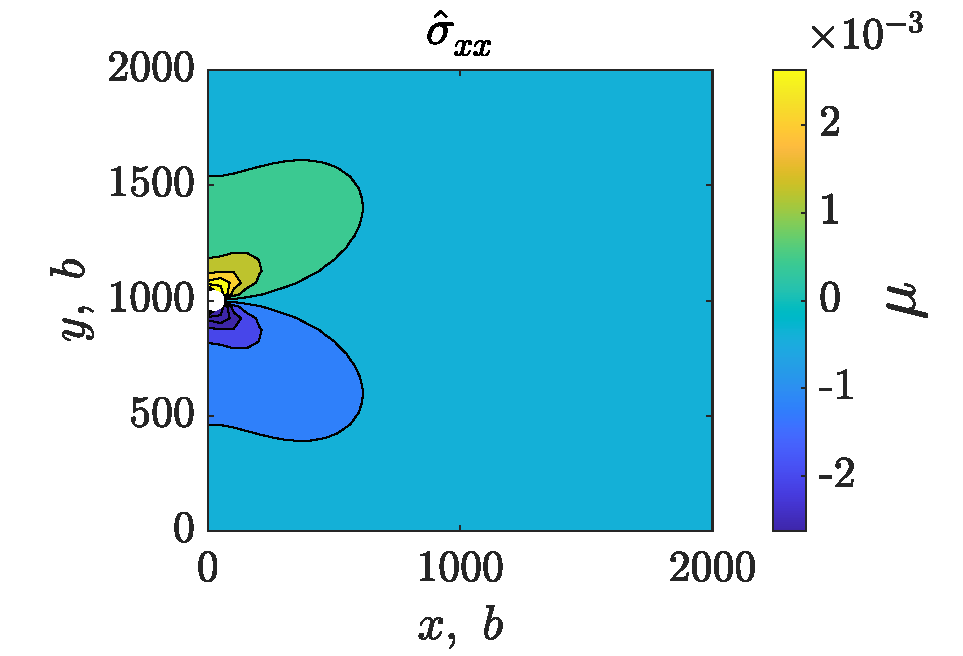
\includegraphics[width=0.3\linewidth]{images/sxxEperp.pdf}}
    }~
    \subfloat[$\hat{\sigma}^\textrm{A}_{xx}$.\label{sf:sxxAeperp}]
    {
        {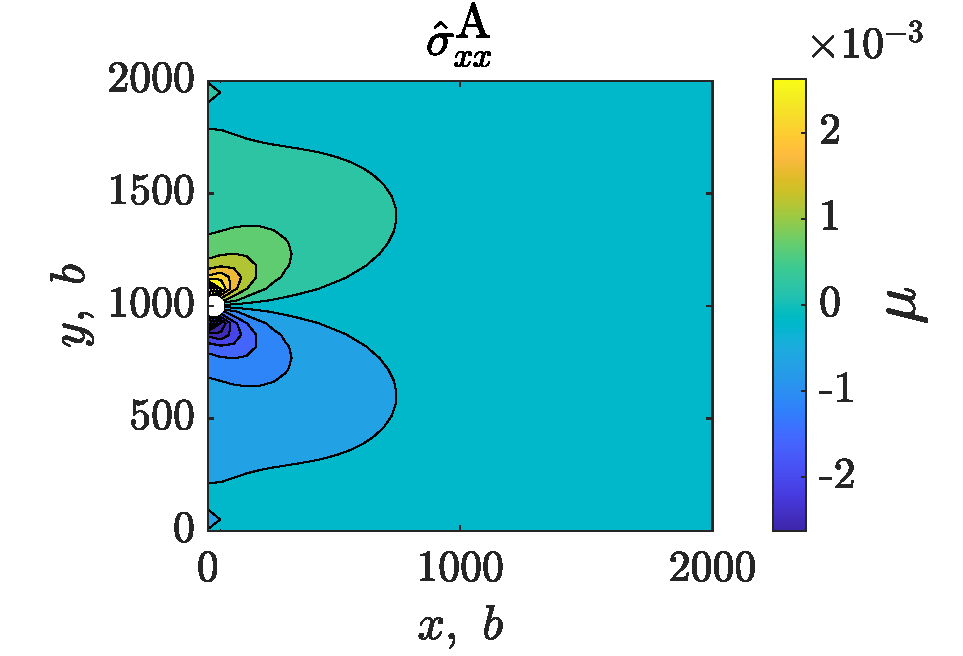
\includegraphics[width=0.3\linewidth]{images/sxxAEperp.pdf}}
    }~
    \subfloat[$\hat{\sigma}^\textrm{N}_{xx}$.\label{sf:sxxNeperp}]
    {
        {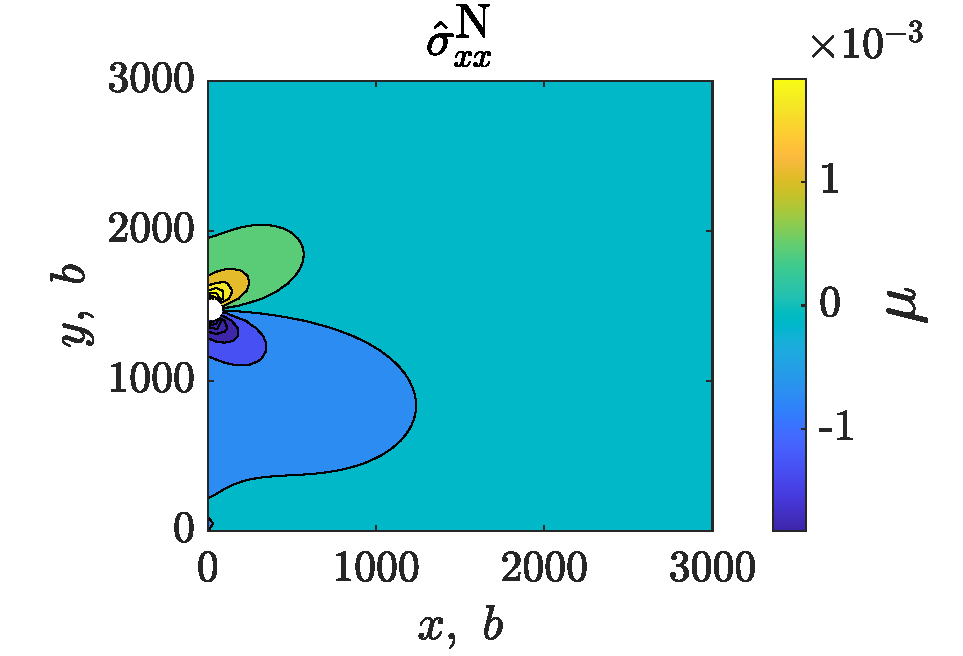
\includegraphics[width=0.3\linewidth]{images/sxxNEperp.pdf}}
    }

    \subfloat[$\hat{\sigma}_{yy}$.\label{sf:syyeperp}]
    {
        {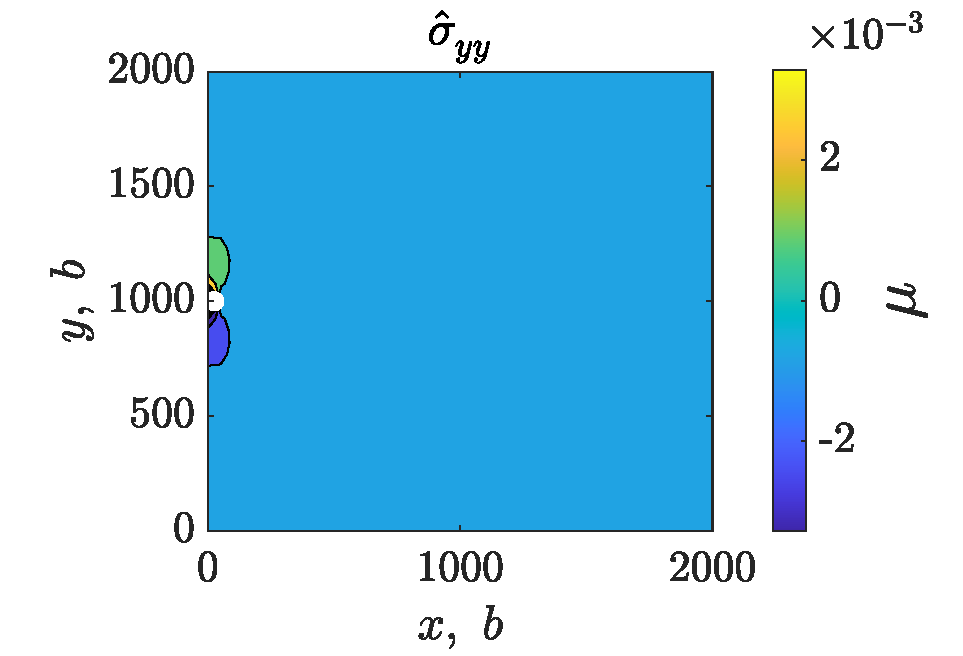
\includegraphics[width=0.3\linewidth]{images/syyEperp.pdf}}
    }~
    \subfloat[$\hat{\sigma}^\textrm{A}_{yy}$.\label{sf:syyAeperp}]
    {
        {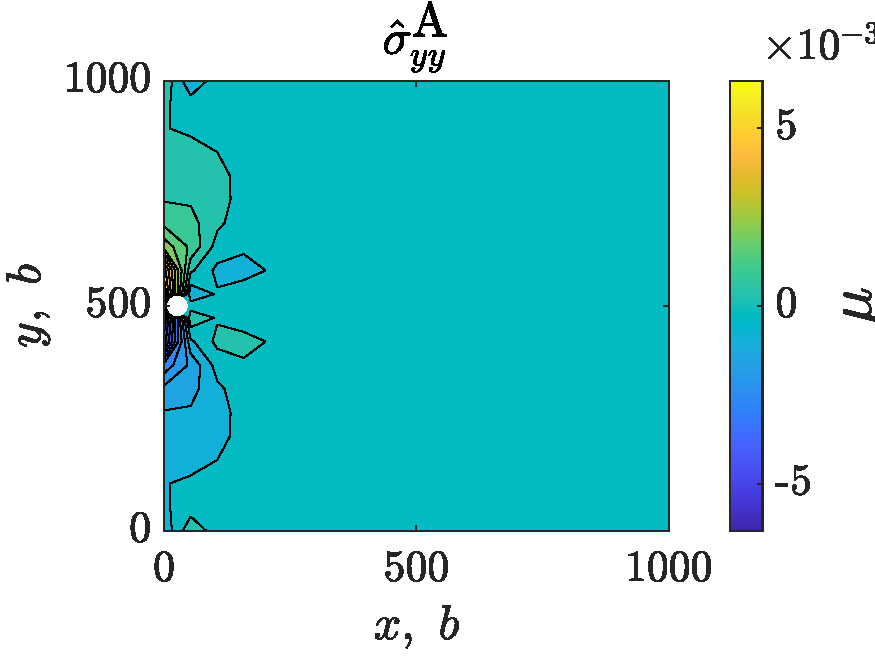
\includegraphics[width=0.3\linewidth]{images/syyAEperp.pdf}}
    }~
    \subfloat[$\hat{\sigma}^\textrm{N}_{yy}$.\label{sf:syyNeperp}]
    {
        {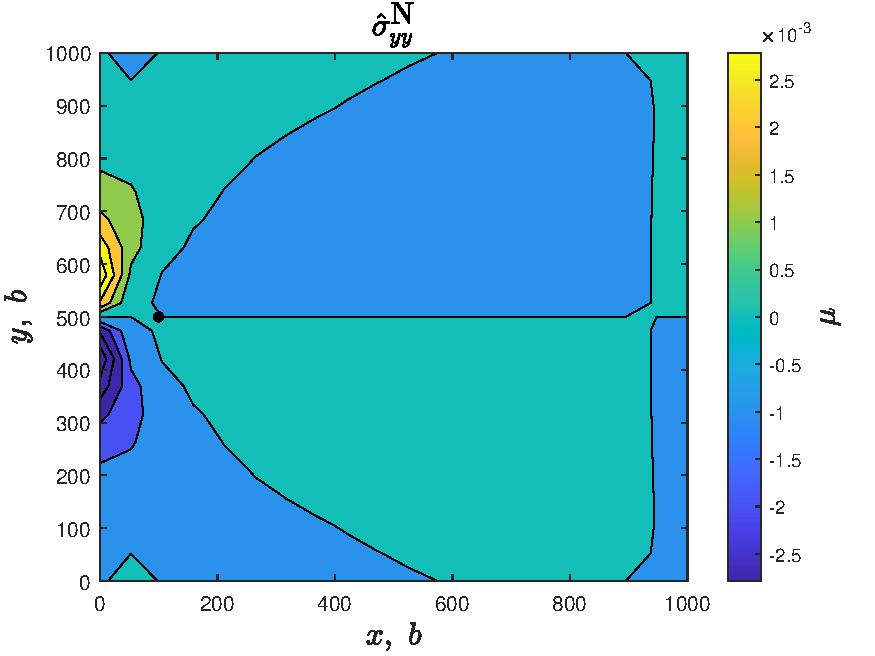
\includegraphics[width=0.3\linewidth]{images/syyNEperp.pdf}}
    }

    \subfloat[$\hat{\sigma}_{xy}$.\label{sf:sxyeperp}]
    {
        {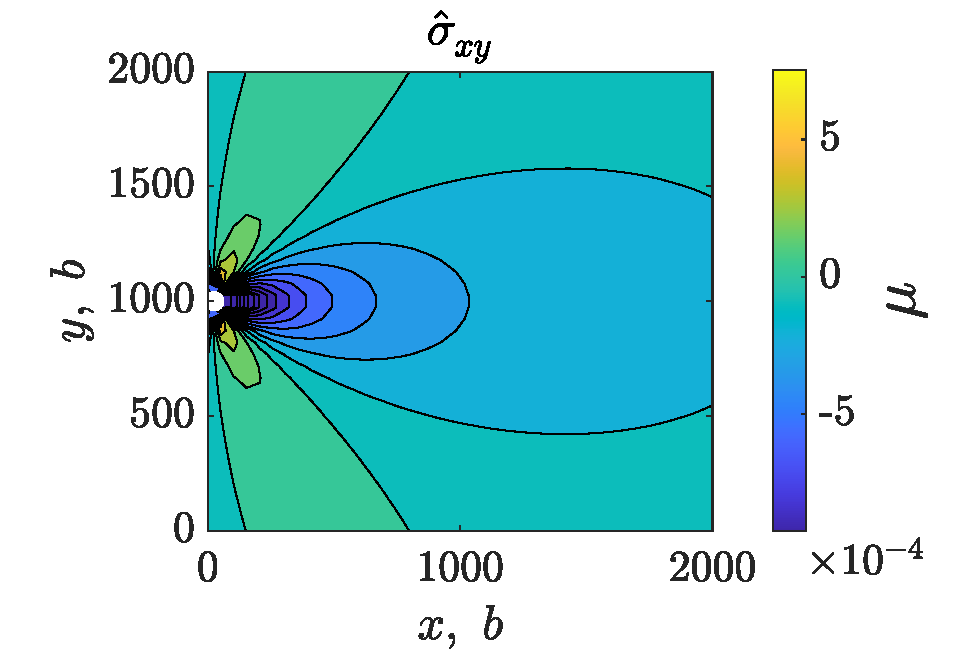
\includegraphics[width=0.3\linewidth]{images/sxyEperp.pdf}}
    }~
    \subfloat[$\hat{\sigma}^\textrm{A}_{xy}$.\label{sf:sxyAeperp}]
    {
        {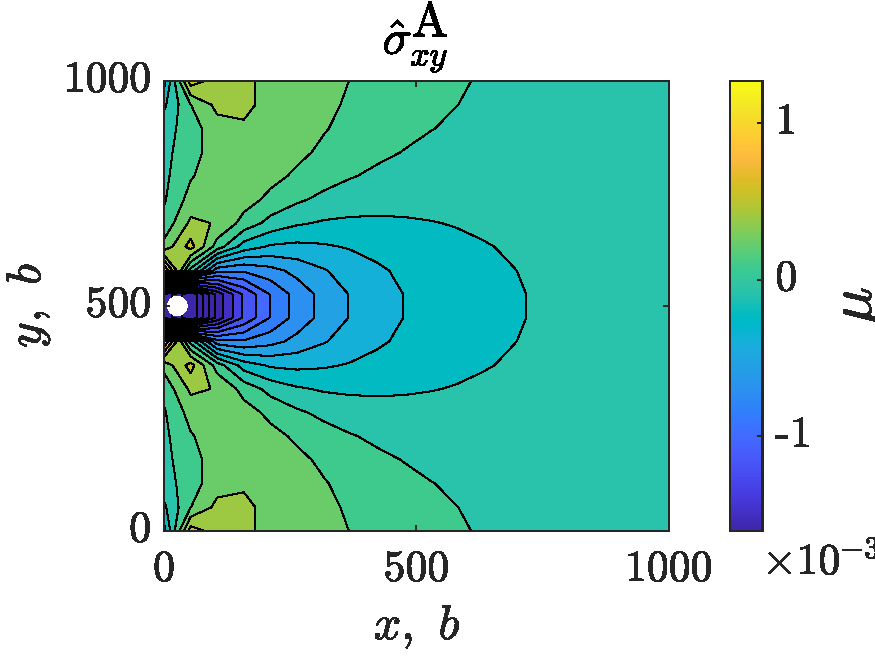
\includegraphics[width=0.3\linewidth]{images/sxyAEperp.pdf}}
    }~
    \subfloat[$\hat{\sigma}^\textrm{N}_{xy}$.\label{sf:sxyNeperp}]
    {
        {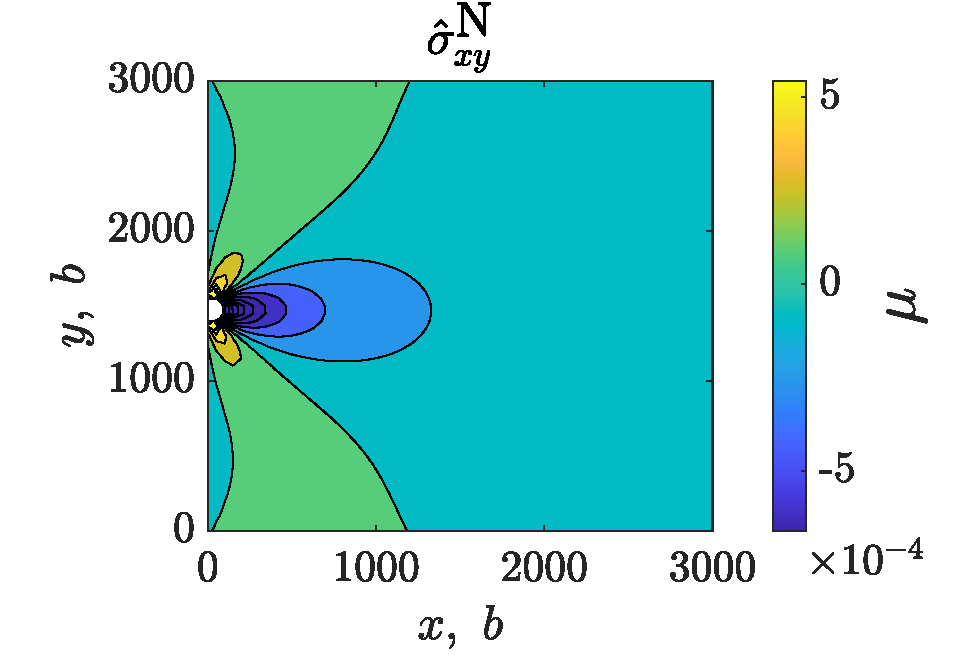
\includegraphics[width=0.3\linewidth]{images/sxyNEperp.pdf}}
    }
    \caption{Image stresses for an edge dislocation with $\vec{l} = [0 0 1]$, $\vec{b} = [1 0 0]$, with $a = 10~b$ with coordinates $(26.3158,~ 500)~b$, i.e. the centre of the first FE from the surface at $x=0$, and in the centre of the simulation box from top to bottom. Here $b = \lVert \vec{b} \rVert \equiv 1$.}
    \label{f:head_vs_ana_vs_num_eperp}
\end{figure}

Note the sign inversion just to the right of the dislocation in \cref{sf:sxxNepar} compared to \cref{sf:sxxepar,sf:sxxAepar}. Stresses like those can lead to dislocations being repelled by surfaces and make the dislocation topology more complex than it should, potentially leading to slowdown or gridlock later in the simulation.
\begin{figure}
    \centering
    \subfloat[$\hat{\sigma}_{xx}$.\label{sf:sxxepar}]
    {
        {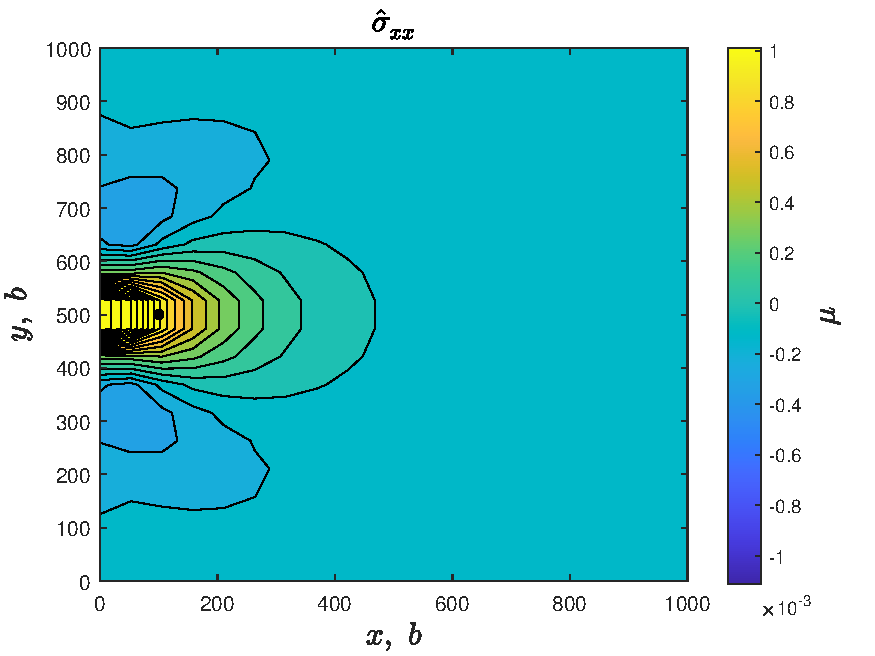
\includegraphics[width=0.3\linewidth]{images/sxxEpar.pdf}}
    }~
    \subfloat[$\hat{\sigma}^\textrm{A}_{xx}$.\label{sf:sxxAepar}]
    {
        {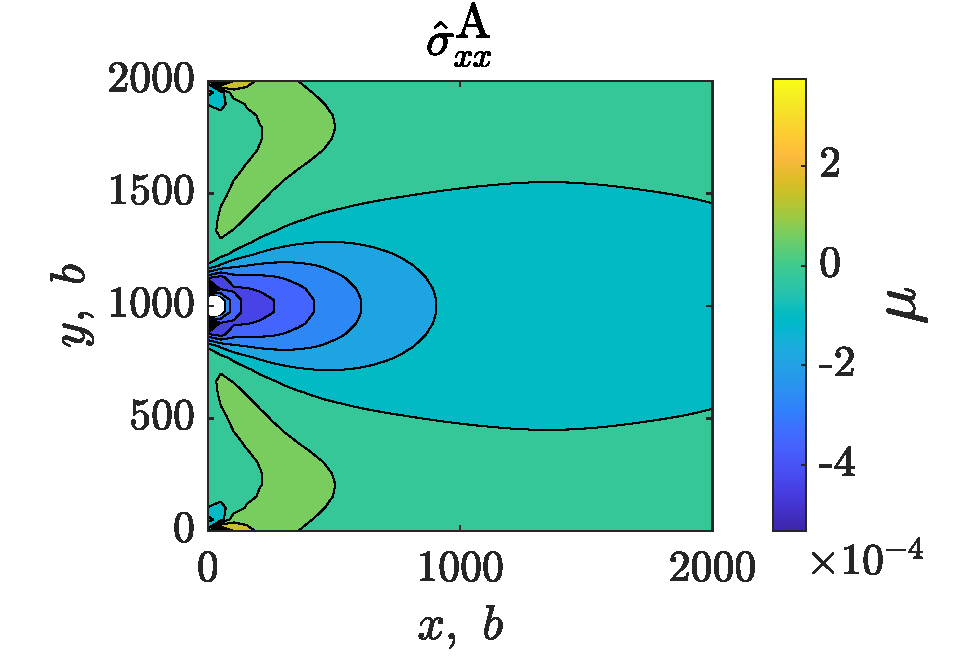
\includegraphics[width=0.3\linewidth]{images/sxxAEpar.pdf}}
    }~
    \subfloat[$\hat{\sigma}^\textrm{N}_{xx}$.\label{sf:sxxNepar}]
    {
        {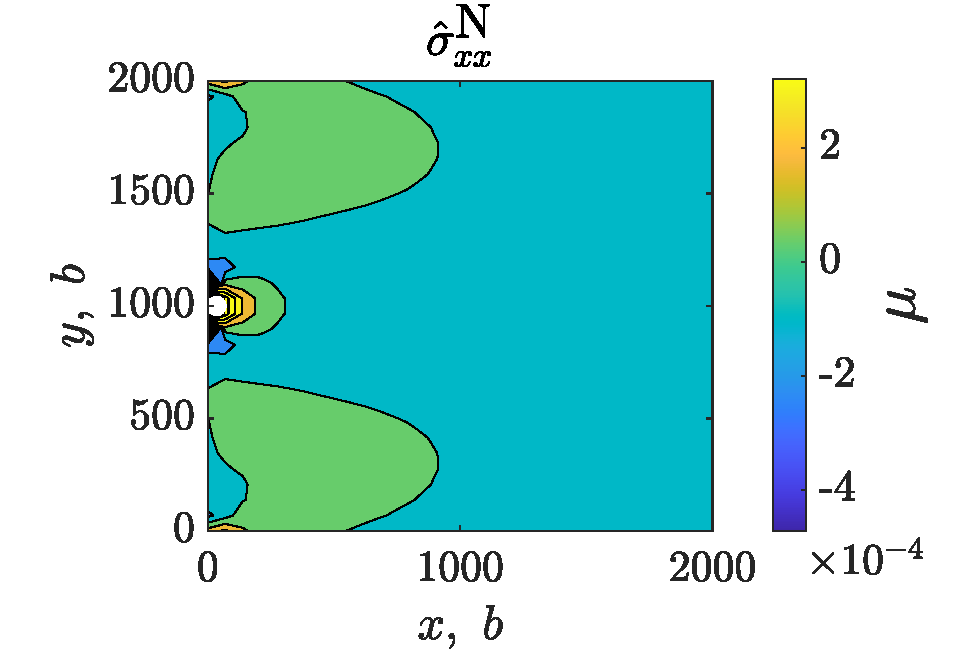
\includegraphics[width=0.3\linewidth]{images/sxxNEpar.pdf}}
    }

    \subfloat[$\hat{\sigma}_{yy}$.\label{sf:syyepar}]
    {
        {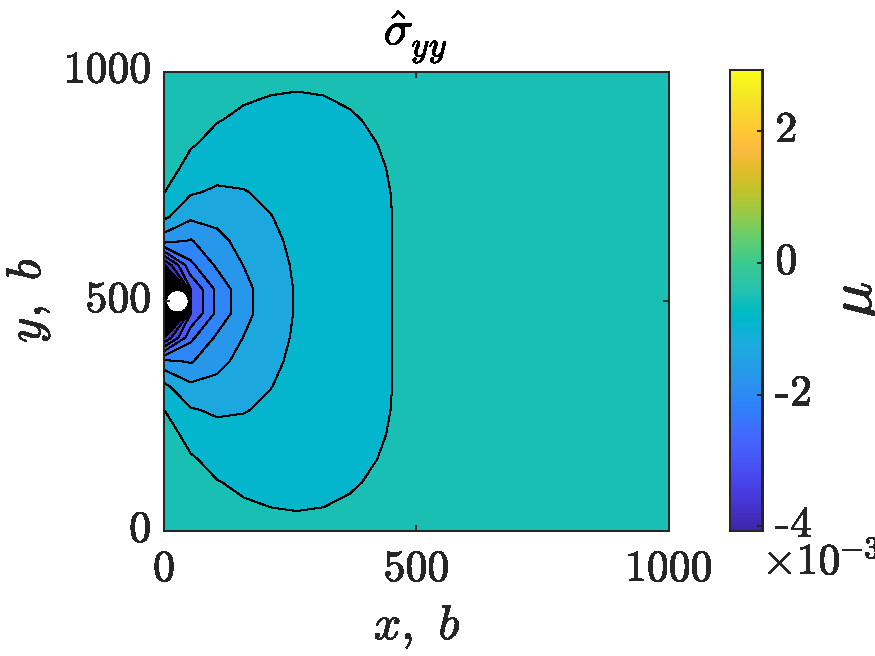
\includegraphics[width=0.3\linewidth]{images/syyEpar.pdf}}
    }~
    \subfloat[$\hat{\sigma}^\textrm{A}_{yy}$.\label{sf:syyAepar}]
    {
        {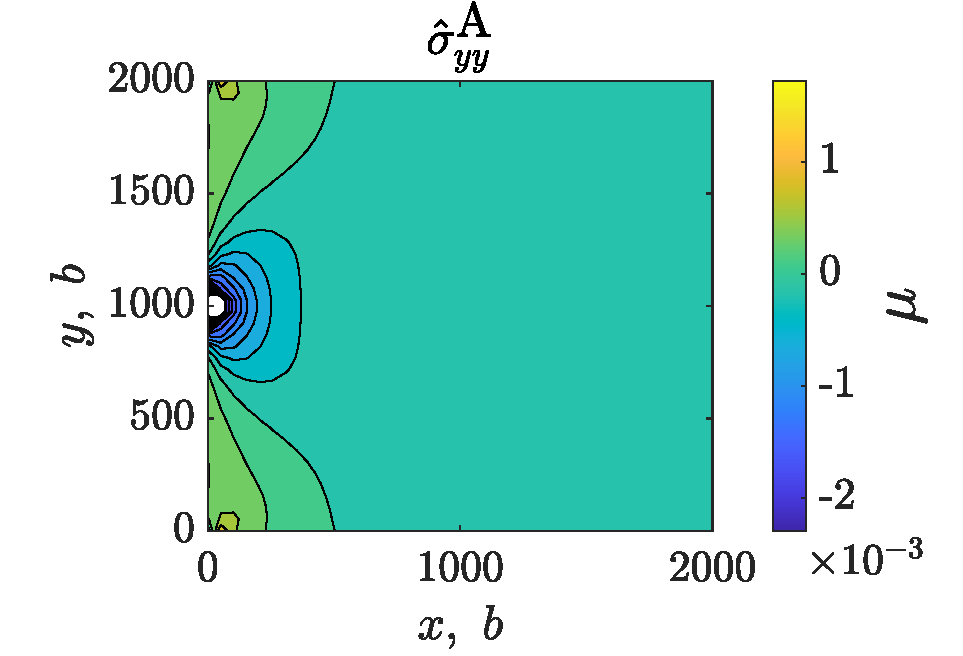
\includegraphics[width=0.3\linewidth]{images/syyAEpar.pdf}}
    }~
    \subfloat[$\hat{\sigma}^\textrm{N}_{yy}$.\label{sf:syyNepar}]
    {
        {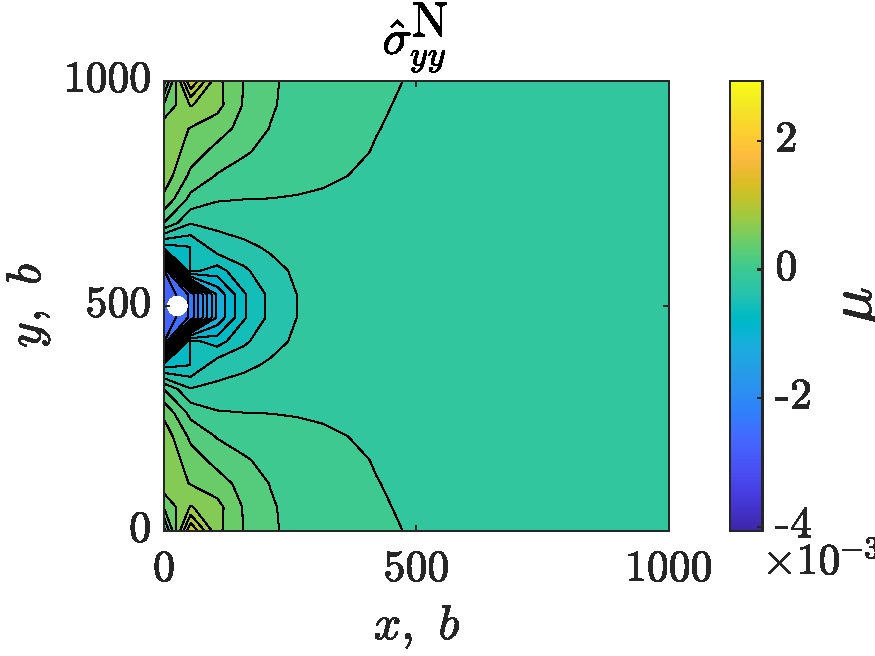
\includegraphics[width=0.3\linewidth]{images/syyNEpar.pdf}}
    }

    \subfloat[$\hat{\sigma}_{xy}$.\label{sf:sxyepar}]
    {
        {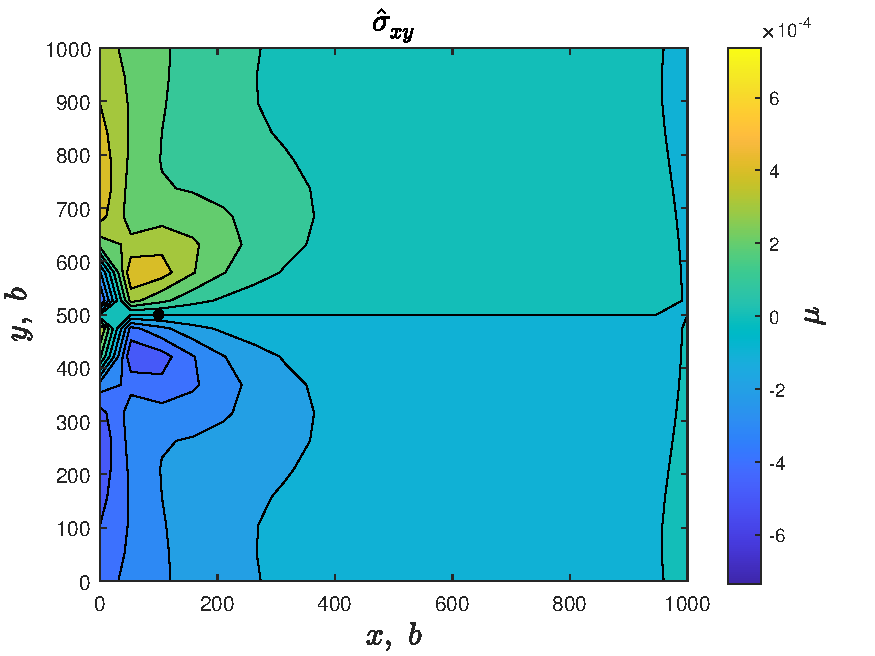
\includegraphics[width=0.3\linewidth]{images/sxyEpar.pdf}}
    }~
    \subfloat[$\hat{\sigma}^\textrm{A}_{xy}$.\label{sf:sxyAepar}]
    {
        {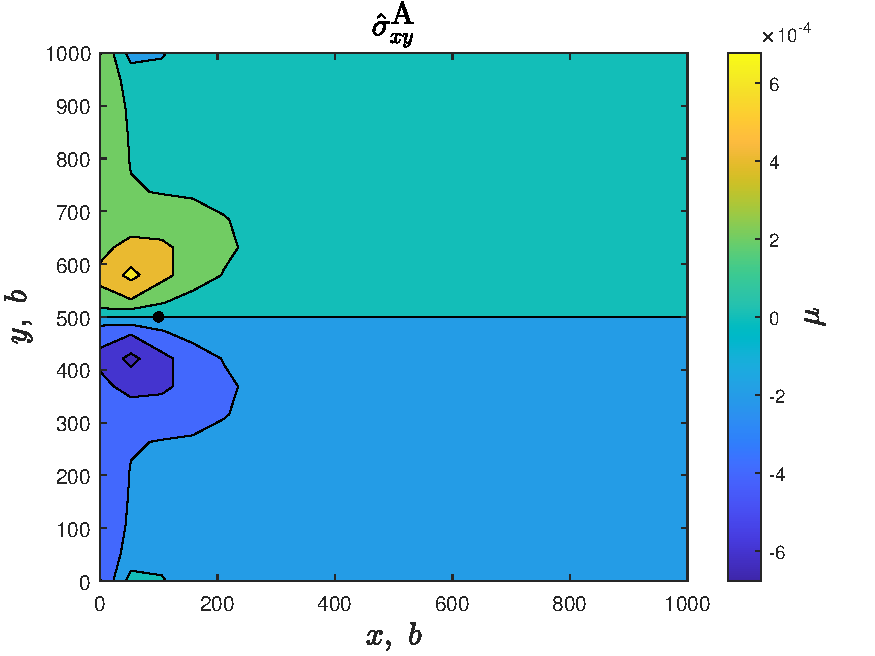
\includegraphics[width=0.3\linewidth]{images/sxyAEpar.pdf}}
    }~
    \subfloat[$\hat{\sigma}^\textrm{N}_{xy}$.\label{sf:sxyNepar}]
    {
        {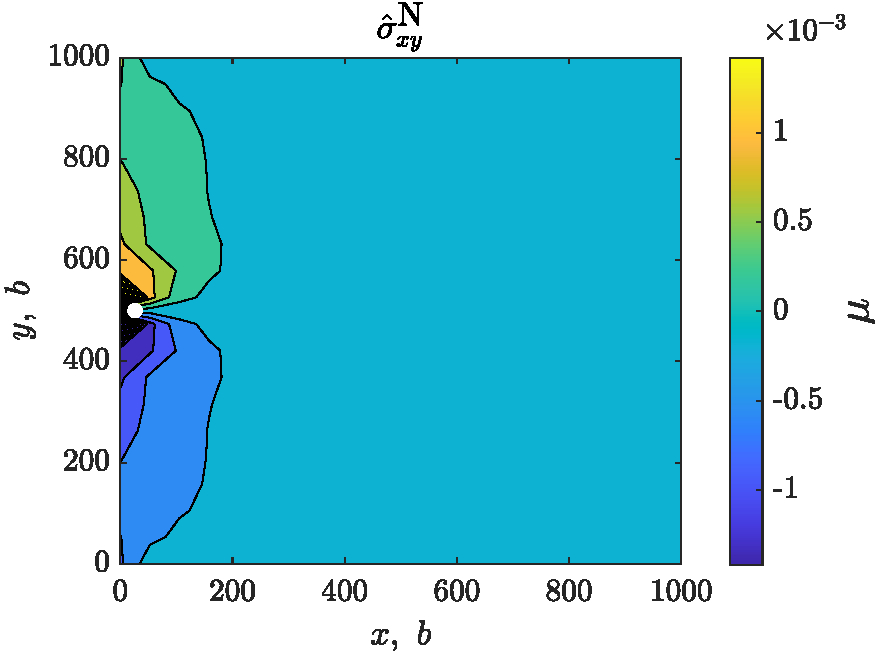
\includegraphics[width=0.3\linewidth]{images/sxyNEpar.pdf}}
    }
    \caption{Image stresses for an edge dislocation with $\vec{l} = [0 0 1]$, $\vec{b} = [0 1 0]$. The rest is the same as \cref{f:head_vs_ana_vs_num_eperp}.}
    \label{f:head_vs_ana_vs_num_epar}
\end{figure}

\begin{figure}
    \centering
    \subfloat[$\hat{\sigma}_{xx}$.\label{sf:sxzscrew}]
    {
        {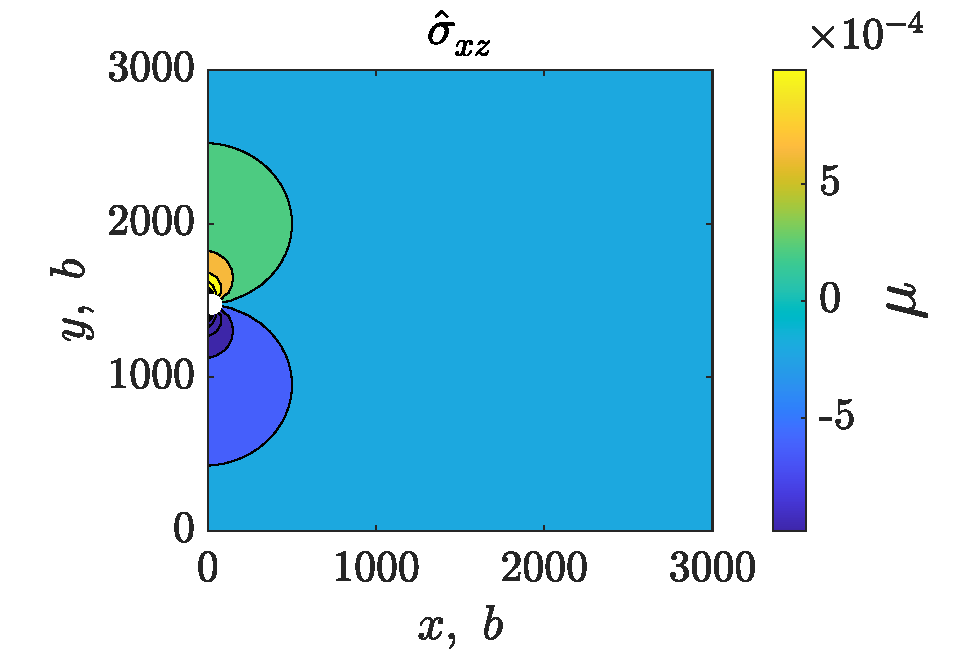
\includegraphics[width=0.3\linewidth]{images/sxzscrew.pdf}}
    }~
    \subfloat[$\hat{\sigma}^\textrm{A}_{xx}$.\label{sf:sxzAscrew}]
    {
        {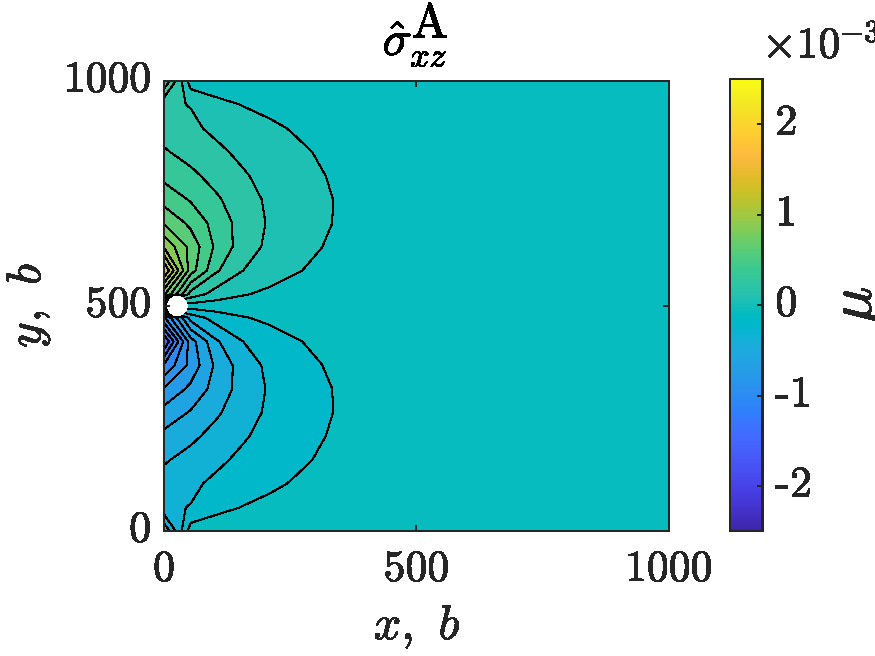
\includegraphics[width=0.3\linewidth]{images/sxzAscrew.pdf}}
    }~
    \subfloat[$\hat{\sigma}^\textrm{N}_{xx}$.\label{sf:sxzNscrew}]
    {
        {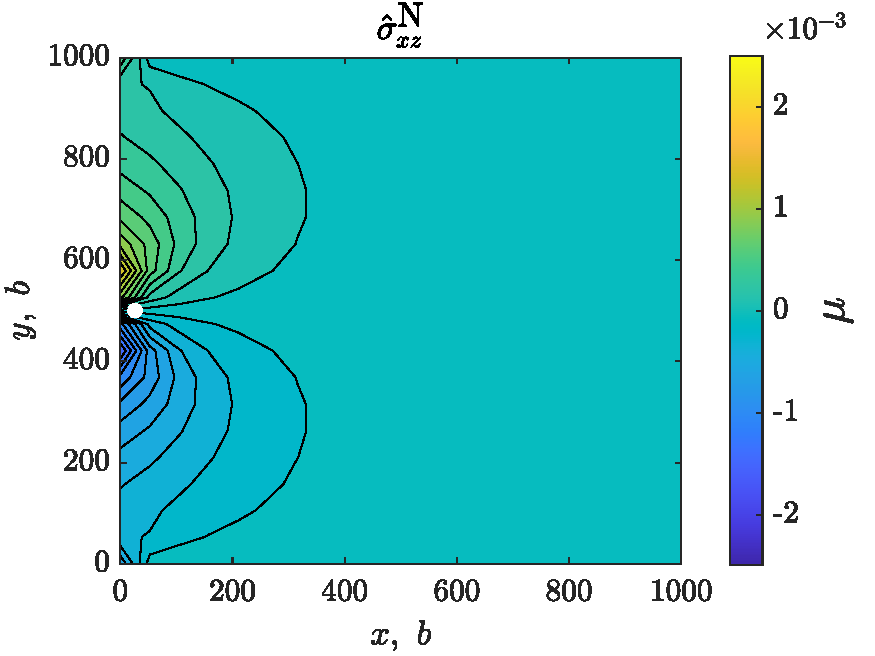
\includegraphics[width=0.3\linewidth]{images/sxzNscrew.pdf}}
    }

    \subfloat[$\hat{\sigma}_{yy}$.\label{sf:szyscrew}]
    {
        {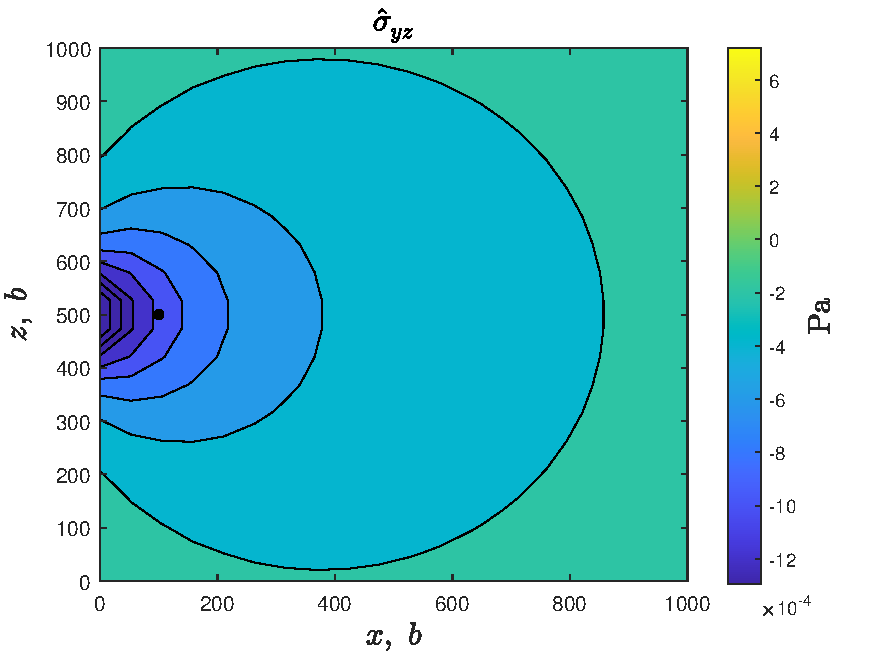
\includegraphics[width=0.3\linewidth]{images/syzscrew.pdf}}
    }~
    \subfloat[$\hat{\sigma}^\textrm{A}_{yy}$.\label{sf:syzAscrew}]
    {
        {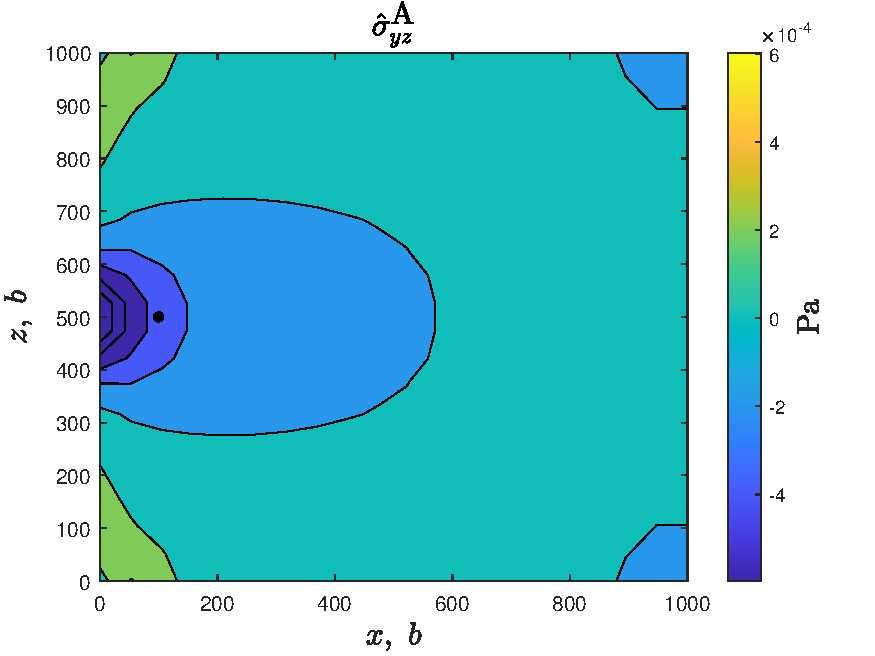
\includegraphics[width=0.3\linewidth]{images/syzAscrew.pdf}}
    }~
    \subfloat[$\hat{\sigma}^\textrm{N}_{yy}$.\label{sf:syzNscrew}]
    {
        {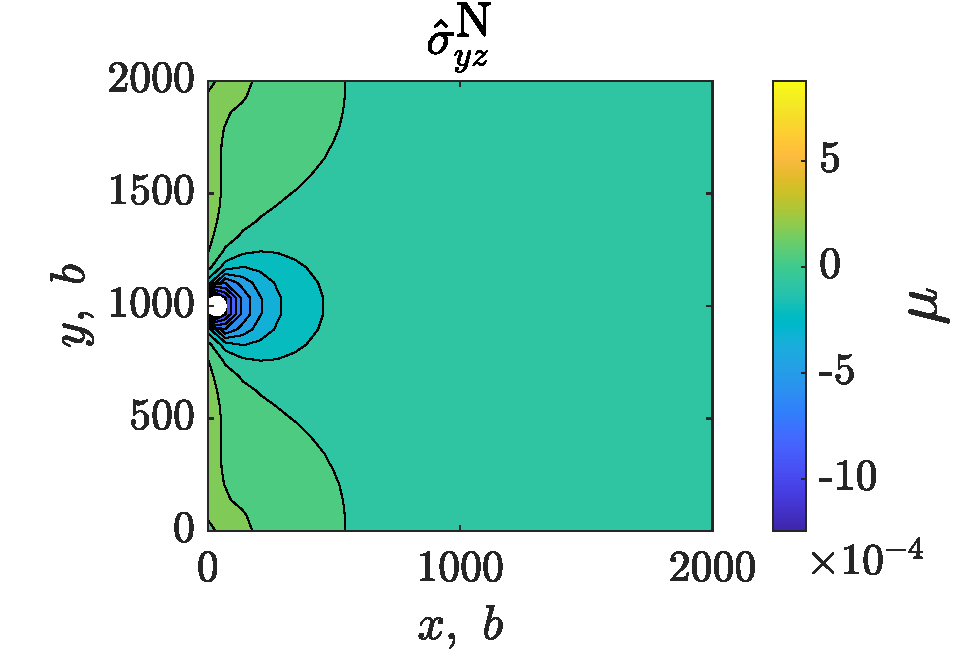
\includegraphics[width=0.3\linewidth]{images/syzNscrew.pdf}}
    }
    \caption{Image stresses for an edge dislocation with $\vec{l} = [0 0 1]$, $\vec{b} = [0 0 1]$. The rest is the same as \cref{f:head_vs_ana_vs_num_eperp}.}
    \label{f:head_vs_ana_vs_num_screw}
\end{figure}

\begin{figure}
    \centering
    \subfloat[$\hat{\sigma}_{xx}$.\label{sf:line_sxxperp}]
    {
        {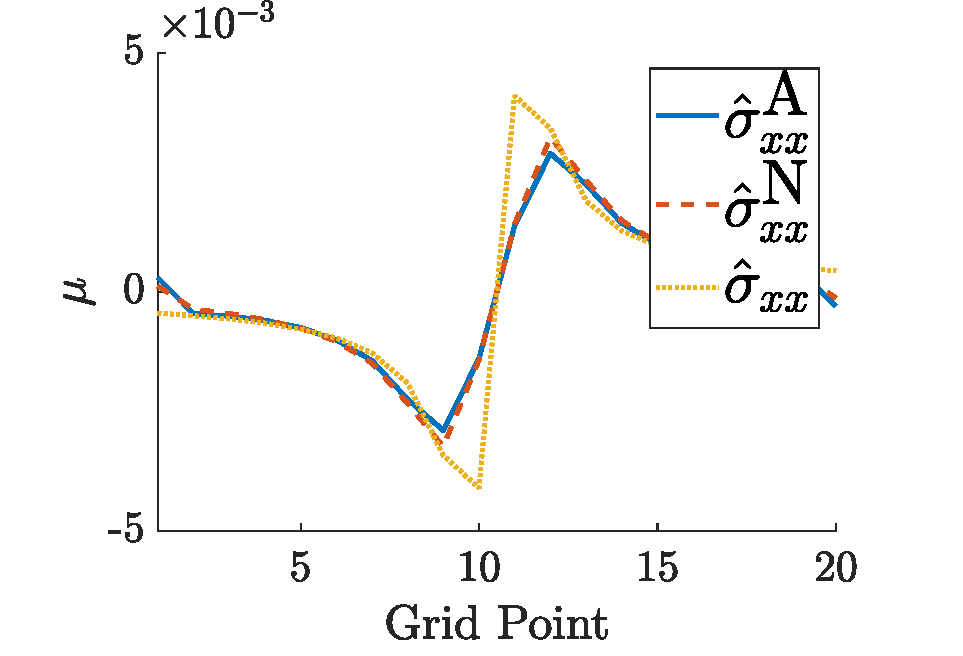
\includegraphics[width=0.3\linewidth]{images/line_sxxEperp.pdf}}
    }~
    \subfloat[$\hat{\sigma}^\textrm{A}_{xx}$.\label{sf:line_syyeperp}]
    {
        {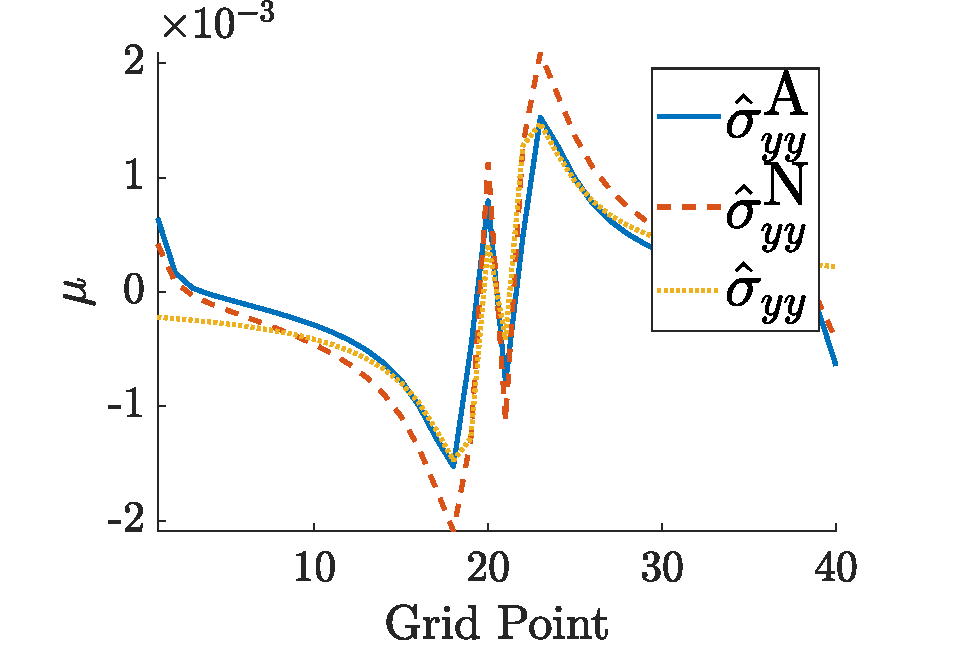
\includegraphics[width=0.3\linewidth]{images/line_syyEperp.pdf}}
    }~
    \subfloat[$\hat{\sigma}^\textrm{N}_{xx}$.\label{sf:line_sxyeperp}]
    {
        {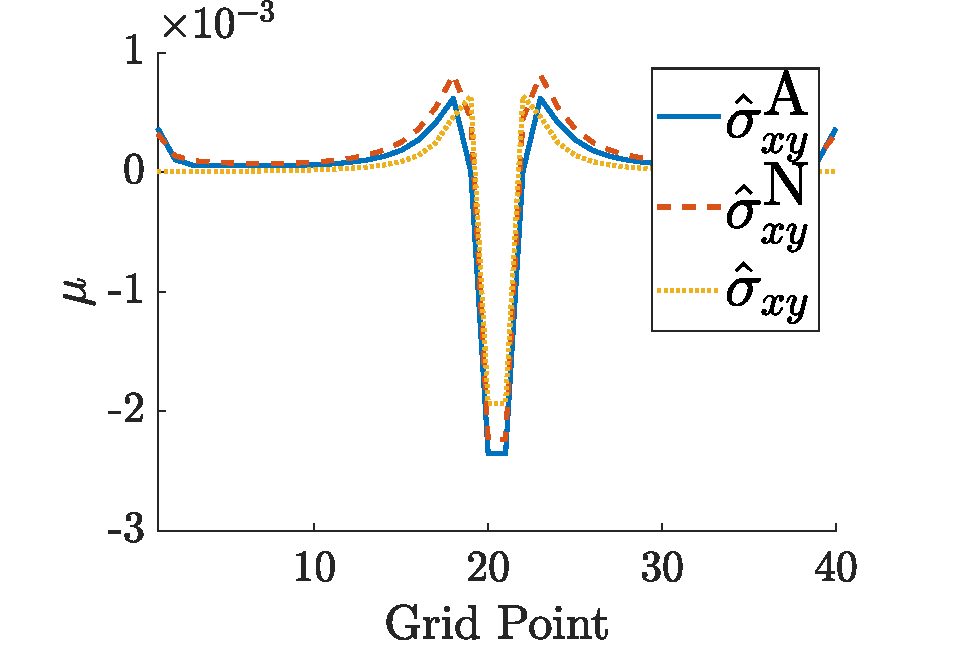
\includegraphics[width=0.3\linewidth]{images/line_sxyEperp.pdf}}
    }

    \subfloat[$\hat{\sigma}_{yy}$.\label{sf:line_sxxepar}]
    {
        {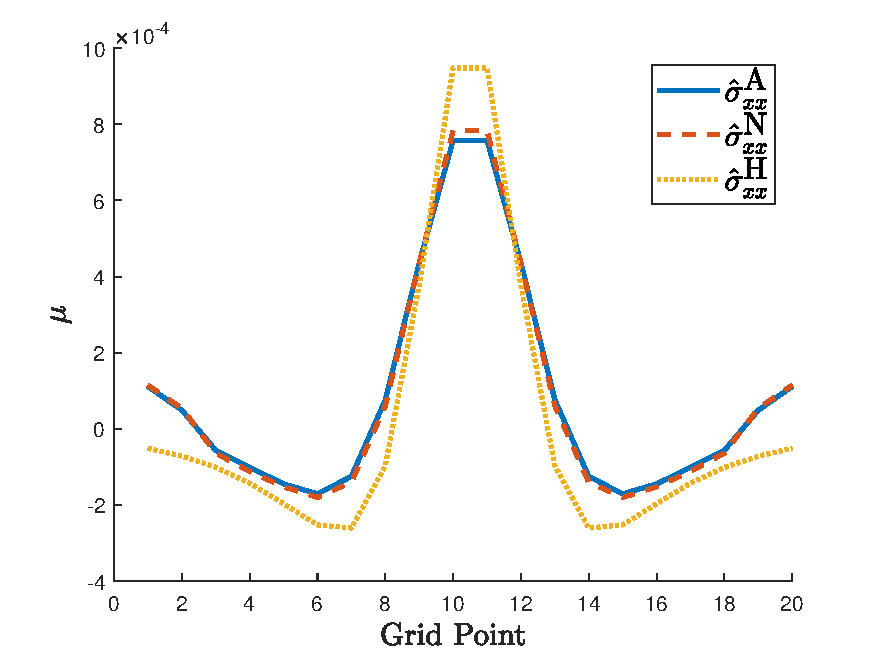
\includegraphics[width=0.3\linewidth]{images/line_sxxEpar.pdf}}
    }~
    \subfloat[$\hat{\sigma}^\textrm{A}_{yy}$.\label{sf:line_syyepar}]
    {
        {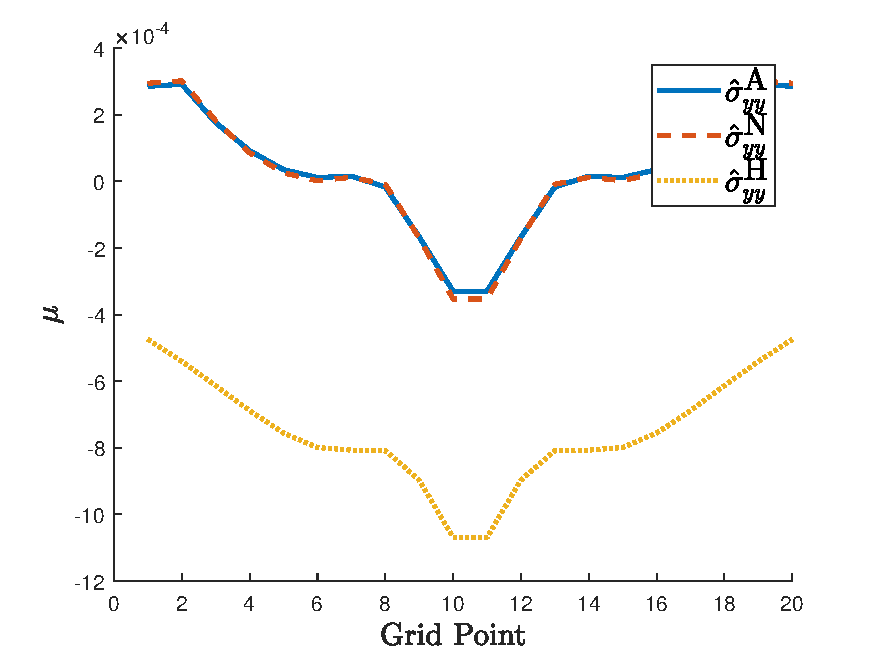
\includegraphics[width=0.3\linewidth]{images/line_syyEpar.pdf}}
    }~
    \subfloat[$\hat{\sigma}^\textrm{N}_{yy}$.\label{sf:line_sxyepar}]
    {
        {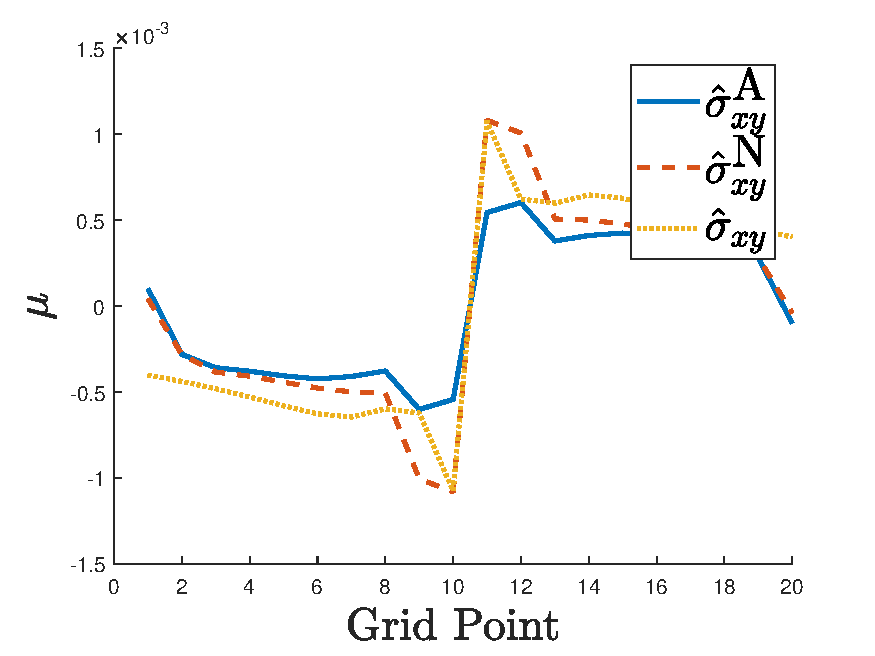
\includegraphics[width=0.3\linewidth]{images/line_sxyEpar.pdf}}
    }

    \subfloat[$\hat{\sigma}_{yy}$.\label{sf:line_sxzscrew}]
    {
        {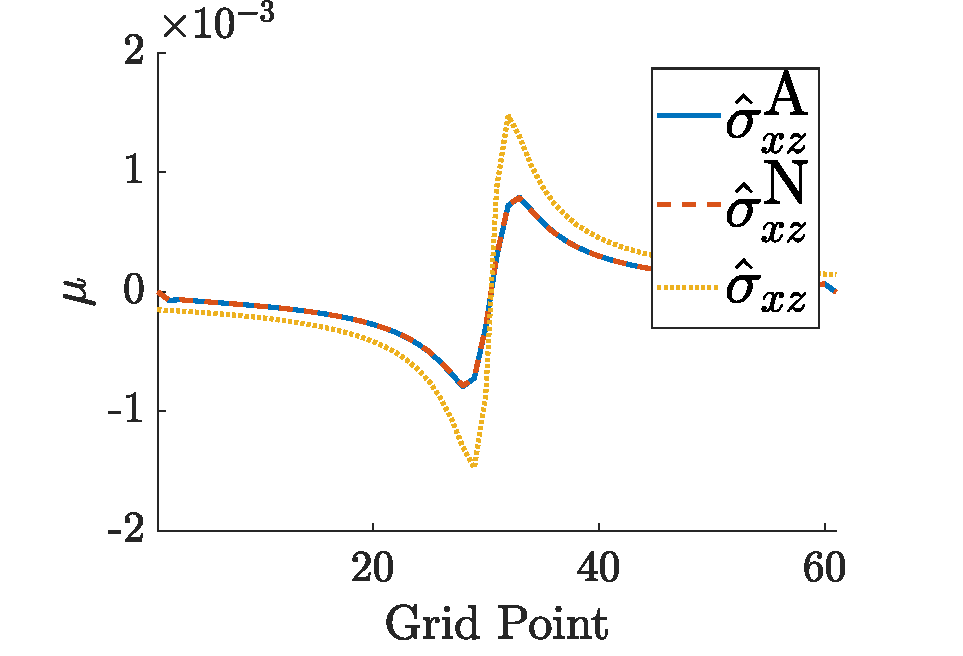
\includegraphics[width=0.3\linewidth]{images/line_sxzscrew.pdf}}
    }~
    \subfloat[$\hat{\sigma}^\textrm{A}_{yy}$.\label{sf:line_syzscrew}]
    {
        {\includegraphics[width=0.3\linewidth]{images/line_syzscrew.pdf}}
    }
    \caption{Line plots of the image stresses at $x = 52.6316\, b$ for the analytic image stresses, as well as those calculated with numeric and analytic tractions. The line corresponds to the first set of nodes away from the boundary at $x = 0$. (a) to (c) correspond to $\vec{b}_{\textrm{e1}}$, (d) to (f) $\vec{b}_{\textrm{e2}}$ and (g) to (h) to $\vec{b}_{\textrm{s}}$.}
    \label{f:head_vs_ana_vs_num_eperp}
\end{figure}
% TODO #28

% In a DDP simulation it is rare to find a dislocation segment so close to a quadrature point that the errors spike so dramatically. However, numerical integration with small $Q$ produces noticeable errors over a wide range of distances and segment lengths. Simulations usually contain a large number of dislocations which are parallel or near-parallel and close to surface elements. \Cref{f:rel_err_par_edge} shows it is not possible to accurately compute the tractions and nodal forces using Gauss quadrature even with a large number of quadrature points.

% It is worth noting that rotational perturbation required for the analytic solution to be non-singular when a dislocation segment is parallel to a surface element can introduce small erroneous force components if the rotation is too large. If the rotational perturbations were small enough and floating point arithmetic exact, these erroneous forces would cancel when averaged over two opposite rotations. We found that a maximum rotation angle of $\pm0.5^\circ$ makes these erroneous force components negligible.

% % TODO #23
% \begin{figure}[t]
%     \centering
%     \includegraphics[width=0.7\linewidth]{images/load_disp.pdf}
%     \caption{Load-displacement curve. When the tractions are evaluated analytically the curve is less noisy compared to numerical integration. As expected the yield point remains the same in both cases.}
%     \label{f:load_disp_curve}
% \end{figure}

% The purpose of the cantilever simulation showed herein is not to be have an exactly physical when it comes to dislocation structure. Our initial source sizes and structure are somewhat unphysical, i.e. square sources with segment lengths on the order of the FE mesh courseness. There are also known issues with junction formation when multiple active slip systems are used in a single simulation. However, we are investigating not only the results but also the robustness and numerical stability of a fully integrated implementation of analytical solutions to dislocation tractions. By throwing the worst case scenario at both numerical and analytic traction calculations, we ensure both numerical and analytic solutions work even when the multiscale nature of the problem causes serious floating point arithmetic errors.

% TODO #22 
% A full discrete dislocation plasticity simulation of a microcantilever bend test demonstrates the benefits of using the analytic solution over numerical integration. The FE nodal forces were evaluated using Gauss quadrature with a single integration point for one simulation, and analytical tractions for the other. The simulations were otherwise identical with a finite element size of $0.25\mu\textrm{m}$ and sixty initial sources equally distributed on the 12 $\{1\bar{1}0\}\langle111\rangle$ bcc slip systems randomly distributed inside the region occuping the central $70\%$ of the cantilever ensuring the simulation proceeded at an acceptable rate and avoiding dislocations from exiting the fixed end, which can lead to problems due to the necessary FEM boundary conditions. The beam was fixed at $x=0$ and displaced by $U_{z}=-0.15~\mu\textrm{m}$ at $x=L=15~\mu\textrm{m}$. The material parameters were those of bcc tungsten, $\mu = 145\,\textrm{GPa}$ and $\nu = 0.28$. The analytic solution significantly reduced the noise in the load displacement curve as shown in \cref{f:load_disp_curve}.

% The inset in \cref{f:load_disp_curve} shows the yield point remains the same, but the reaction forces diverge from each other as the simulation progresses. It should be noted that the dislocation structure was unchanged and so the change in the mechanical response is due entirely to the accuracy of the force calculation. The fluctuations are due to dislocations approaching a free surface and generating a large traction which is suddenly removed when the segment exits. These events are difficult to capture accurately when using numerical integration.

% The dislocation structure did not change much in either case. In fact, when looking at it from the zoom level of \cref{f:dln_struc}, they both appear identical. There are however, many small differences in node position. Surprisingly, depending on the specific simulation, we have found between $10--20\%$ less dislocation segments when the analytic solution is used. Meaning the numerical solution systematically underestimates the average contribution of every single dislocation segment, with occasional massive spikes in force when a dislocation nears a gauss point. We expect these differences to get larger as simulation runtime increases. This is a fundamental and practically unavoidable problem of the numerical solution.

% % TODO #24
% \begin{figure}[t]
%     \centering
%     \includegraphics[width=0.7\linewidth]{images/analytic_struct.pdf}
%     \caption{Final dislocation structure using analytic tractions.}
%     \label{f:dln_struc}
% \end{figure}

% There are a few things that determine whether the numerical solutions are good enough for a given problem. When primarily investigating larger scale features of a dislocation structure---such as larger scale investigation of dislocation forresting around inclusions---Gauss quadrature is quite suitable. However, if one is interested in investigating the finer details of a dislocation structure---such as the nuanced interactions with closly packed inclusions---the analytic method is best. Furthermore, when investigating load-displacement curves, the analytical solutions provide a much better description for a relatively small increase in computational cost \cite{Queyreau}. That being said, the cost is nowhere near rate limiting, segment-segment forces and topological changes quickly become much more expensive as they both have worse asymptotic scaling, and topological changes also quickly become memory bound. An accurate description of load-displacement curves should also implement the exact displacement boundary conditions obtained by \citet{ddd_disp}.

All our subsequent simulations have used analytic tractions as they run faster and yield more reasonable dislocation structures, particularly for more complex simulations.

\section{Acknowledgements}

We would like to thank Prof. Sylvain Queyreau and Lawrence Livermore National Laboratory for their invaluable input. This work was supported by the Consejo Nacional de Ciencia y Tecnologia, Fondo Sectorial CONACYT-Secretaria de Energia-Sustentabilidad Energetica Cuarto Periodo [291129]. This work was supported by the Engineering and Physical Sciences Research Council Centre for Doctoral Training in the Science and Technology of Fusion Energy EP/L01663X/1 and Fellowship grant EP/N007239/1.
%% References
%%
%% Following citation commands can be used in the body text:
%% Usage of \cite is as follows:
%%   \cite{key}          ==>>  [#]
%%   \cite[chap. 2]{key} ==>>  [#, chap. 2]
%%   \citet{key}         ==>>  Author [#]

%% References with bibTeX database:
\newcommand{\newblock}{}
\bibliographystyle{unsrtnat}
\bibliography{references.bib}

%% Authors are advised to submit their bibtex database files. They are
%% requested to list a bibtex style file in the manuscript if they do
%% not want to use model1-num-names.bst.

%% References without bibTeX database:

% \begin{thebibliography}{00}

%% \bibitem must have the following form:
%%   \bibitem{key}...
%%

% \bibitem{}

% \end{thebibliography}
\end{document}

%%
%% End of file `elsarticle-template-1-num.tex'.